\documentclass[lettersize,journal]{IEEEtran}

% ========== Key Modification: Use \documentclass with direct font configuration ==========
\usepackage[T1]{fontenc}
\usepackage{times}
% ========== End Key Modification ==========

\usepackage{amsmath,amsfonts}
\usepackage{algorithmic}
\usepackage{algorithm}
\usepackage{array}
\usepackage[caption=false,font=normalsize,labelfont=sf,textfont=sf]{subfig}
\usepackage{textcomp}
\usepackage{stfloats}
\usepackage{url}
\usepackage{verbatim}
\usepackage{graphicx}
\usepackage{cite}
\usepackage{caption}
\usepackage{booktabs}
\captionsetup{justification=centering}
\usepackage{tikz}
\usepackage{booktabs}
\usepackage{multirow}
\usepackage[hidelinks]{hyperref}
\usetikzlibrary{shapes.geometric, arrows, positioning, fit, backgrounds, shadows}

\usepackage{tikz}
\usetikzlibrary{arrows.meta, positioning, calc, shapes.geometric}

\hyphenation{op-tical net-works semi-conduc-tor IEEE-Xplore}


\begin{document}

\title{FA-DCG: A Plug-and-Play Feature-Level Frequency-Aware Dilated Convolution Module for Single-Channel SAR Flood Segmentation}

%IEEE Publication Technology,~\IEEEmembership{Staff,~IEEE,

%This paper was produced by the IEEE Publication Technology Group. They are in Piscataway, NJ.

%\author{Yanmei Zhang, Yun Su,  Xiaoqiang Jia*}

%\thanks{This paper was produced by the IEEE Publication Technology Group. They are in Piscataway, NJ.}
%\thanks{Manuscript received April 19, 2021; revised August 16, 2021.}}



\author{
    Yanmei Zhang\thanks{Yanmei Zhang: 2139501391@qq.com},
    Xiaoqiang Jia\thanks{Xiaoqiang Jia (Correspondence) -- jiaxiaoqiang@imut.edu.cn}*,
    Yun Su\thanks{Yun Su: suyun@imut.edu.cn},
\thanks{School of Information Engineering, Inner Mongolia University of Technology, Hohhot 010051, China}}

\maketitle

\begin{abstract}
In single-channel SAR flood segmentation, preprocessed images often still contain residual interference and weak texture regions, making discriminative features difficult to extract. To address this, we propose the Frequency-Aware Dilated Convolution with Gating (FA-DCG) module, which performs enhancement at the feature level. FA-DCG consists of two components. First, a learnable channel-wise dilation preference assigns each channel a soft combination of multi-scale receptive fields according to its frequency characteristics, enabling the network to capture both fine boundaries and homogeneous water bodies. Second, a response-selective gating mechanism recalibrates the dilated channel responses, strengthening discriminative features and suppressing false activations caused by residual interference. The module is lightweight, introducing parameter increases of only 6.4\% on FCN and 1.7\% on U-Net, and can be plugged into existing CNN architectures. On a flood-event-isolated SAR dataset, FA-DCG improves the mIoU of an FCN baseline from 0.6319 to 0.8243, and a U-Net baseline from 0.7048 to 0.8782. Leave-one-region-out cross-validation yields an average mIoU improvement from 0.6084 to 0.8156, confirming generalization across unseen regions. Feature visualizations on both architectures show enhanced intra-class consistency and suppressed false activations. Across three random seed repetitions, all metric standard deviations remain below 0.02.
\end{abstract}


\begin{IEEEkeywords}
Synthetic Aperture Radar (SAR), Flood Segmentation, Frequency-Aware Dilated Convolution, Adaptive Gating, Feature Enhancement, Residual Interference Suppression
\end{IEEEkeywords}



\section{Introduction}

\IEEEPARstart{S}{ynthetic} Aperture Radar (SAR) can work day and night and see through clouds and rain, making it very useful for rapid flood mapping \cite{Amitrano2024RemoteSens}. From 2000 to 2018, more than 900 flood events were recorded worldwide, affecting about 255 to 290 million people \cite{Tellman2021Nature}. Quickly and accurately extracting flooded areas is a key need for disaster response and assessment \cite{Lv2022RemoteSens}. The technical scenario studied in this paper is: flood water segmentation from a single post-disaster single-channel SAR intensity image. In this scenario, there is no pre-disaster reference image for change detection \cite{Bai2021RemoteSens}, nor polarization or optical bands to help. The input that can be reliably obtained is usually just one single-channel backscatter intensity image.

The lack of information brings two related difficulties. The first is the remaining speckle noise. Multiplicative speckle comes from the coherent imaging mechanism of SAR \cite{Wang2025JSTARS_Speckle}. Classic methods like Lee filtering can provide effective preprocessing \cite{Farhadiani2024ISPRS}, but these filters use a fixed intensity smoothing strategy that is not learned from data. Their parameters cannot be adjusted for the downstream segmentation task \cite{Zhao2024JSTARS_Filter}, and they may blur water-land boundaries while suppressing noise. The second is the lack of clear clues. A single-channel intensity image only records the backscatter intensity of ground objects. The intensity values of water, dry sand, smooth roads, and radar shadow areas overlap heavily \cite{Ritushree2023MIGARS, Liu2022JSTARS, Tian2022RemoteSens}. It is hard to make a reliable decision using only local gray values. This lack of information makes the problems of remaining speckle noise and weak clues even more serious \cite{Huang2024JSTARS}. These difficulties appear as: many holes and fragments inside flooded areas due to speckle \cite{Gao2025AppSci}, and unclear water-land boundaries \cite{Zhao2024MGRS}. Also, labeling SAR images is costly, so there are usually not enough labeled samples for training \cite{Zortea2023IEEE}. The core problem of this paper can thus be stated as: how to improve the ability to distinguish weak features and effectively suppress remaining noise under limited samples. The labels used in this paper correspond to flooded water areas identified by visual interpretation from post-disaster SAR images. The goal is to directly extract flooded areas from a single post-disaster image \cite{Amer2025RemoteSens}, without using multi-temporal comparison or external water masks.

For pixel-level semantic segmentation, general deep networks already provide solid baseline architectures. From FCN \cite{Long2015CVPR} to the encoder-decoder design of U-Net \cite{Ronneberger2015MICCAI}, and then to Swin Transformer \cite{Liu2021ICCV} which uses hierarchical self-attention to keep global modeling ability while reducing computation, feature modeling accuracy has been steadily improved. However, these designs follow the principle of treating all spatial positions and feature channels equally. This principle works well for natural images but shows a structural problem for single-channel SAR flood images. On one hand, large flooded areas need broad information gathering to bridge speckle holes and form a confident decision that the area is water. On the other hand, narrow river channels, small water patches, and fuzzy water-land boundaries need fine spatial resolution to locate boundaries accurately \cite{Tan2023RemoteSens}. A fixed receptive field strategy—whether it is CNN gradually expanding receptive field by stacking layers, or Transformer using fixed window partitioning for attention—couples these two conflicting needs in one processing flow, making it hard to satisfy both.

To address this problem, some works have tried to let networks allocate attention more flexibly at the architecture level. Li and Kong \cite{Li2023RemoteSensing} added channel and spatial attention modules to the DeepLabv3+ framework to refine decoder features, showing the benefit of attention in SAR water segmentation. However, that method focuses on weighting spatial positions and does not adjust the receptive field scale itself. Wang et al. \cite{Wang2022NLCANet} introduced asymmetric pyramid non-local blocks and channel attention to capture long-range dependencies, making up for the lack of global context. Yet this still stays at the level of looking farther, without treating boundaries and homogeneous areas differently in terms of receptive field. Shen et al. \cite{Shen2024ELLKNet} proposed an adaptive kernel selection mechanism, where the convolution kernel scale can be adjusted based on input content. This moves from adjusting spatial coverage to adjusting the receptive field scale. But the kernel selection weights are shared across space, and do not clearly separate the different receptive field needs of homogeneous areas versus boundaries. Wang et al. \cite{Wang2025NRSANet} further included speckle statistics in the design, building a scattering-aware dynamic attention and a noise-boundary diffusion module to reduce noise while protecting boundaries. That work organizes receptive field allocation mainly for noise suppression, but does not systematically model receptive field needs based on differences in spatial frequency. These methods gradually improve the ability to adjust receptive field dynamically, but always focus on spatial attention. They do not directly address a basic fact: homogeneous flooded areas are dominated by low-frequency structure, while boundaries and small water bodies are dominated by high-frequency details. The need for receptive field size is structurally different between these two. Spatial attention can tell the network where to focus, but not at what scale to focus. Lacking this ability is a key obstacle to further improving segmentation accuracy. Zortea et al. \cite{Zortea2023IEEE} provide supporting evidence from another angle: using synthetic flood events to train a compact U-Net achieves good segmentation accuracy with far fewer parameters. This shows that a lightweight approach is practical under small sample conditions. This means any module designed to improve feature discrimination must strictly limit added parameters, otherwise trainability under small samples will be reduced.

Parallel to spatial methods, another direction is to use frequency domain processing. In wavelet-based methods, He et al. \cite{He2024GRSL} used wavelet decomposition for multi-scale feature learning to suppress speckle, and Jamali et al. \cite{Jamali2024IJAG} combined wavelet transform with residual learning for dual-polarization SAR flood detection. These works show the basic feasibility of combining frequency decomposition and convolutional networks. However, wavelet methods have a built-in constraint: the basis functions are chosen before training starts, and the frequency band division is fixed during training and inference. This means the frequency decomposition strategy does not adapt to the task or the input content. To go beyond this limit, later works tried to learn frequency and spatial information together at the network architecture level. Depo-Net \cite{DepoNet2025} designed frequency-domain self-attention and spatial-frequency co-modulation modules. FSA-SARNet \cite{Zhou2026FSA-SARNet} explicitly adds a frequency-domain feature extraction branch that works in parallel with a spatial branch. S3T-Net \cite{Yang2025S3T} combines a frequency-domain encoding unit with a vision transformer to capture local texture and reduce noise sensitivity. These methods achieve clear accuracy gains on several public SAR datasets, showing the benefit of frequency-spatial co-design. But at the same time, their designs share a common feature: they all add an explicit frequency transform branch, such as wavelet decomposition modules, frequency-domain self-attention, or spatial-frequency two-stream interaction. This leads to two direct consequences. First, the number of model parameters increases accordingly. With enough labeled samples, this added complexity may bring performance gains. But when training samples are limited to tens or hundreds of images, too many learnable parameters increase the risk of overfitting—the model tends to memorize specific texture patterns in the training data instead of learning generalizable features for water detection. Second, the added frequency branch means the method is not simply plug-and-play. Its deployment and tuning require extra hyperparameter design. It is worth noting that Turkmenli et al. \cite{Turkmenli2024HistSegNet} proposed a different lightweight idea: embedding a histogram extraction layer into the segmentation network, achieving IoU gains with almost no added learnable parameters. That work shows lightweight enhancement is possible, but it captures global gray value statistics and does not yet have the ability to adaptively respond at the spatial frequency level.

Besides mining information from the SAR image itself, using external priors is another promising path. Garg et al. \cite{Garg2024RSE} combined VV/VH dual-polarization features with topographic prior, effectively improving flood boundary identification in low-contrast areas like deserts. Li et al. \cite{Li2026JournalofHydrology} used consistency with a hydrodynamic model to constrain network training, achieving 90.2\% overall accuracy under limited labels. These works show that external priors can effectively compensate for the lack of information in weak-texture areas of a single-channel intensity image. However, in the scenario considered in this paper, dual-polarization data, topographic elevation information, and hydrodynamic model outputs are often not available or cannot be obtained quickly. The input that can be reliably obtained is usually just one single-channel intensity image. This practical limitation means that methods relying on explicit frequency transform branches or multi-source external priors face applicability problems when directly moved to our scenario.

Based on the above analysis, this paper tries to answer the following question: For single-channel SAR flood water segmentation, is it possible to design a feature enhancement module that meets all of these conditions at once—can sense different spatial frequency components and allocate receptive field accordingly, does not rely on explicit frequency transform branches or multi-source external data, and adds very few learnable parameters so that it remains trainable under small samples and can be used as a plug-and-play module? The answer to this question may start from a basic property of dilated convolution. The dilation rate essentially determines the spatial frequency bandwidth sampled by the convolution layer \cite{Chen2024CVPR}: a larger dilation rate gives sparser sampling points, and the extracted features tend to reflect broad structural information; a smaller dilation rate gives denser sampling points, and the extracted features tend to reflect local details. Following this reasoning, if different channels in the same convolution layer can each learn their own preference for dilation rate, then each channel can naturally choose to respond to a specific frequency range. Furthermore, if these dilation rate preferences are automatically determined during training via backpropagation, the network can decide for itself which channels to set with a large receptive field for context aggregation, and which channels to set with a small receptive field for boundary detail \cite{Hu2023SAMDConv}. This approach sets the control granularity for frequency sensing at the feature level rather than the pixel level. The learnable parameters are reduced from pixel-level to channel-level, and no explicit transform branches are needed—frequency sensing is implicitly embedded in the sampling pattern of the dilated convolution itself, not in an added functional module.

Based on this idea, this paper proposes a Feature-level frequency-Aware Dilated Convolution Gating module (FA-DCG). The module has three tightly connected components: (1) per-channel dilation rate selection, which softly selects the most suitable dilation rate for each input channel from a predefined set of scales; (2) multi-scale feature extraction, where convolution kernels with different dilation rates process their corresponding channels to produce multi-scale feature responses; (3) adaptive gating, which recalibrates the responses of each channel, enhancing feature components that are useful for segmentation and suppressing remaining speckle noise and uncertainty in weak-texture areas. FA-DCG is designed as a plug-and-play module that can be easily added to existing segmentation backbones, with very few additional learnable parameters.

The main contributions of this paper are summarized as follows:
\begin{enumerate}
\item We propose the FA-DCG module, which implicitly embeds feature-level frequency sensing into per-channel learnable dilation rate selection and adaptive gating. It achieves adaptive multi-scale receptive field allocation without adding explicit frequency transform branches or relying on external prior data.
\item We design an adaptive gating mechanism that recalibrates the multi-scale feature responses of each channel, effectively suppressing remaining speckle noise and discrimination uncertainty in weak-texture areas of single-channel SAR intensity images.
\item We systematically evaluate the effectiveness, generalization ability, and plug-and-play nature of the proposed module on a self-built SAR flood segmentation dataset, with strict flood-event-based partitioning, multi-seed repeated experiments, leave-one-region cross-validation, integration tests with two backbone networks, and comparison with representative baseline methods.
\end{enumerate}

The rest of this paper is organized as follows. Section II describes the detailed design of the FA-DCG module and the overall network architecture. Section III describes the experimental dataset, settings, and implementation details. Section IV reports the experimental results. Section V discusses the findings. Section VI concludes the paper.



\section{Methodology}

\subsection{Problem Definition}

The objective of the single-channel SAR image flood segmentation task is to accurately identify flood areas from the input SAR image. Given a single-channel SAR image $I \in \mathbb{R}^{1 \times H \times W}$, the model needs to predict the corresponding binary segmentation mask $M \in \{0,1\}^{H \times W}$, where a pixel value of 1 denotes the flood class and 0 denotes the background. The core challenge of this task lies in the fact that despite Lee filtering being applied in the preprocessing stage for initial denoising, issues such as residual speckle noise, blurred water boundaries, and insufficient contrast in weak-texture regions persist in the SAR images. Coupled with limited labeled samples, it becomes difficult for the model to establish stable discriminative criteria.

This paper adopts Fully Convolutional Network (FCN) and U-Net as the baseline models. FCN replaces the fully connected layers in traditional CNNs with convolutional layers, enabling it to accept arbitrarily sized input images and produce segmentation outputs with the same spatial resolution as the input. U-Net employs a symmetric encoder-decoder structure, fusing multi-scale features through skip connections to restore spatial details. Both baseline models employ the binary cross-entropy loss function, calculated pixel-wise between the predicted probability and the ground truth label:

\begin{equation}
\mathcal{L}_{\text{BCE}} = -\frac{1}{N}\sum_{i=1}^{N}\left[y_i \log(\hat{y}_i) + (1-y_i)\log(1-\hat{y}_i)\right]
\end{equation}
where $N$ denotes the total number of image pixels, $y_i$ is the ground truth label of the $i$-th pixel, and $\hat{y}_i$ represents the predicted flood probability from the model.

\subsection{FA-DCG Module Design}

The Feature-Level Frequency-Aware Dilated Convolution Module with Adaptive Gating (FA-DCG) is designed to enhance the feature representation capability of single-channel SAR images through a feature-level frequency-aware mechanism while maintaining a plug-and-play profile. As illustrated in Fig. \ref{fig:fa_dcg}, the module comprises two core components: a Learnable Channel-wise Dilation Preference and a Response-Selective Gating Mechanism.



\begin{figure}[t]
    \centering
    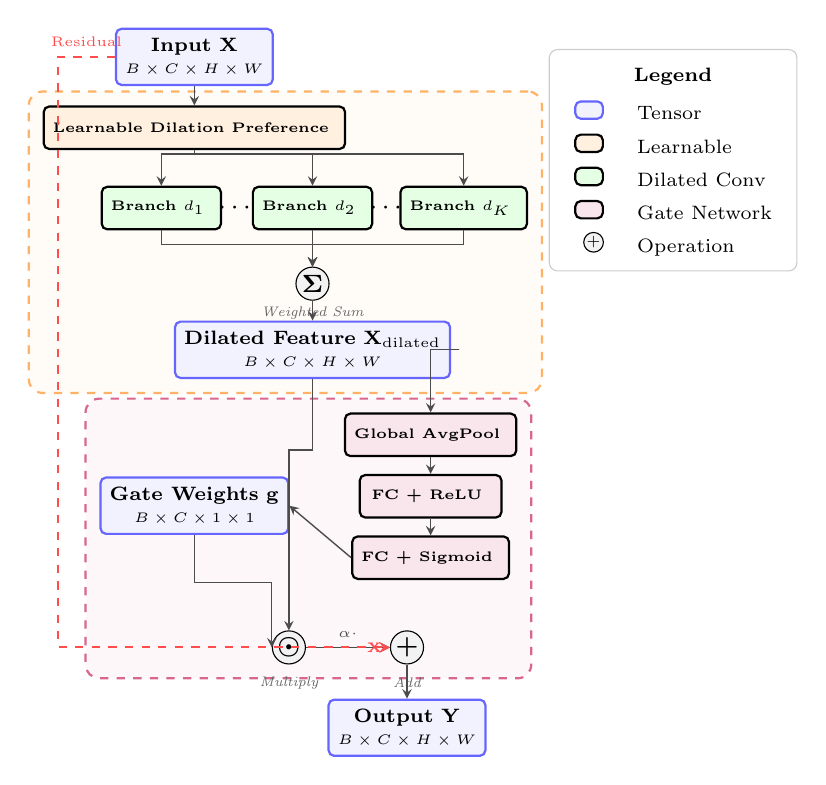
\begin{tikzpicture}[
        box/.style={
            rectangle, 
            draw=black, 
            line width=0.8pt, 
            minimum width=1.8cm,      
            minimum height=0.54cm,    
            align=center, 
            font=\tiny\bfseries,      
            rounded corners=2pt
        },
        tensor/.style={
            rectangle, 
            draw=blue!60, 
            fill=blue!5, 
            line width=0.8pt, 
            minimum width=1.7cm,      
            minimum height=0.48cm,    
            align=center, 
            font=\scriptsize,
            rounded corners=2pt
        },
        smallbox/.style={
            rectangle, 
            draw=black, 
            line width=0.8pt, 
            minimum width=1.45cm,     
            minimum height=0.54cm,    
            align=center, 
            font=\tiny\bfseries,
            rounded corners=2pt
        },
        op/.style={
            circle, 
            draw=black, 
            fill=gray!10, 
            inner sep=0pt, 
            minimum size=0.42cm,      
            font=\small\bfseries
        },
        arrow/.style={
            ->, 
            >=stealth, 
            line width=0.5pt, 
            color=black!70
        },
        dashedarrow/.style={
            ->, 
            >=stealth, 
            line width=0.7pt, 
            color=red!70, 
            dashed
        },
        label/.style={
            font=\tiny\itshape, 
            text=black!60
        }
    ]

    % ===== Stage 1 Blocks =====
    \node[tensor] (input) at (-1.5, 2.4) {
        \textbf{Input} $\mathbf{X}$ \\
        \tiny $B \times C \times H \times W$
    };

    \node[box, fill=orange!12] (learn_d) at (-1.5, 1.5) {
        \textbf{Learnable Dilation Preference}
    };

    \node[smallbox, fill=green!10] (conv1) at (-1.92, 0.48) {
        \textbf{Branch} $d_1$
    };

    \node[smallbox, fill=green!10] (conv2) at (0, 0.48) {
        \textbf{Branch} $d_2$
    };

    \node[smallbox, fill=green!10] (conv3) at (1.92, 0.48) {
        \textbf{Branch} $d_K$
    };

    \node[font=\normalsize] at (-0.96, 0.48) {$\cdots$};
    \node[font=\normalsize] at (0.96, 0.48) {$\cdots$};

    \node[op] (sum) at (0, -0.48) {$\boldsymbol{\Sigma}$};
    \node[label] at (0, -0.85) {\tiny Weighted Sum};

    \node[tensor] (mid_tensor) at (0, -1.32) {
        \textbf{Dilated Feature} $\mathbf{X}_{\text{dilated}}$ \\
        \tiny $B \times C \times H \times W$
    };

    % ===== Stage 2 Blocks =====
    \node[tensor] (gate) at (-1.5, -3.3) {
        \textbf{Gate Weights} $\mathbf{g}$ \\
        \tiny $B \times C \times 1 \times 1$
    };

    \node[box, fill=purple!10] (pool) at (1.5, -2.4) {
        \textbf{Global AvgPool}
    };

    \node[box, fill=purple!10] (fc1) at (1.5, -3.18) {
        \textbf{FC + ReLU}
    };

    \node[box, fill=purple!10] (fc2) at (1.5, -3.96) {
        \textbf{FC + Sigmoid}
    };

    \node[op] (mul) at (-0.3, -5.1) {$\boldsymbol{\odot}$};
    \node[label] at (-0.3, -5.55) {\tiny Multiply};

    \node[op] (add) at (1.2, -5.1) {$\boldsymbol{+}$};
    \node[label] at (1.2, -5.55) {\tiny Add};

    \node[tensor] (output) at (1.2, -6.12) {
        \textbf{Output} $\mathbf{Y}$ \\
        \tiny $B \times C \times H \times W$
    };

    % ===== Arrows =====
    \draw[arrow] (input.south) -- (learn_d.north);
    \draw[arrow] (learn_d.south) -- ++(0, -0.05) -| (conv1.north);
    \draw[arrow] (learn_d.south) -- ++(0, -0.05) -| (conv2.north);
    \draw[arrow] (learn_d.south) -- ++(0, -0.05) -| (conv3.north);
    \draw[arrow] (conv1.south) -- ++(0, -0.18) -| (sum.north);
    \draw[arrow] (conv2.south) -- ++(0, -0.18) -| (sum.north);
    \draw[arrow] (conv3.south) -- ++(0, -0.18) -| (sum.north);
    \draw[arrow] (sum.south) -- (mid_tensor.north);
    
    % 修正: Dilated Feature 到 Global AvgPool - 先右再向下折
   \draw[arrow] (mid_tensor.east) -- ++(0.1, 0) -| (pool.north);
    
    \draw[arrow] (pool.south) -- (fc1.north);
    \draw[arrow] (fc1.south) -- (fc2.north);
    
    % FC + Sigmoid 到 Gate Weights - 直线连接
    \draw[arrow] (fc2.west) -- (gate.east);
    
    \draw[arrow] (mid_tensor.south) -- ++(0, -0.9) -- ++(-0.3, 0) -- (mul.north);
    \draw[arrow] (gate.south) -- ++(0, -0.6) -| (mul.west);
    \draw[arrow] (mul.east) -- (add.west) 
        node[midway, above, font=\tiny] {$\alpha \cdot$};
    \draw[arrow] (add.south) -- (output.north);
    \draw[dashedarrow] (input.west) -- ++(-0.72, 0) 
        node[midway, above, font=\tiny\color{red!80}] {Residual} 
        |- (add.west)
        node[pos=0.95, right, font=\tiny\color{red!80}] {$\mathbf{X}$};

    % ===== Stage Backgrounds =====
    \begin{scope}[on background layer]
        \node[draw=orange!60, fill=orange!3, rounded corners=5pt, line width=0.8pt, dashed,
              fit=(learn_d) (conv1) (conv3) (sum) (mid_tensor), 
              inner sep=5pt, 
              label={[orange!80, font=\scriptsize\bfseries]north west:{Stage 1: Feature-Level Multi-Scale Dilated Fusion}}] {};
        
        \node[draw=purple!60, fill=purple!3, rounded corners=5pt, line width=0.8pt, dashed,
              fit=(pool) (fc1) (fc2) (gate) (mul) (add), 
              inner sep=5pt, 
              label={[purple!80, font=\scriptsize\bfseries]north west:{Stage 2: Response-Selective Gating}}] {};
    \end{scope}

    % ===== Legend (字体放大为 \scriptsize，图标相应放大) =====
    \node[draw=gray!40, fill=white, rounded corners=3pt, inner sep=3pt,
          anchor=north west] at (3.0, 2.5) {
        \begin{tabular}{rl}
        \multicolumn{2}{c}{\scriptsize\bfseries Legend} \\[2pt]
        \tikz \node[tensor, minimum width=0.35cm, minimum height=0.22cm, inner sep=0pt] {}; & \scriptsize Tensor \\
        \tikz \node[box, fill=orange!12, minimum width=0.35cm, minimum height=0.22cm, inner sep=0pt] {}; & \scriptsize Learnable \\
        \tikz \node[smallbox, fill=green!10, minimum width=0.35cm, minimum height=0.22cm, inner sep=0pt] {}; & \scriptsize Dilated Conv \\
        \tikz \node[box, fill=purple!10, minimum width=0.35cm, minimum height=0.22cm, inner sep=0pt] {}; & \scriptsize Gate Network \\
        \tikz \node[op, minimum size=0.25cm, font=\tiny] {$+$}; & \scriptsize Operation \\
        \end{tabular}
    };

    \end{tikzpicture}
    \caption{Architecture of the proposed FA-DCG (Feature-Level Frequency-Aware Dilated Convolution Module with Adaptive Gating). 
    Stage 1 implicitly extracts multi-frequency features by fusing dilated convolutions with learnable channel-wise dilation preferences at the feature level. 
    Stage 2 employs a response-selective gating mechanism to adaptively recalibrate channel responses, which are finally integrated via a residual connection.}
    \label{fig:fa_dcg}
\end{figure}


\subsubsection{Learnable Channel-wise Dilation Preference}

In standard convolutional neural networks, dilated convolutions expand the receptive field by introducing gaps, and the dilation rate is typically kept uniform across all channels. However, different regions in SAR images exhibit distinct frequency characteristics: flood areas generally present relatively uniform textures, corresponding to low-frequency components that require a larger receptive field to capture global context; whereas regions such as boundaries and isolated water bodies contain high-frequency information, requiring a smaller receptive field to preserve spatial precision. Based on this observation, and inspired by FADC \cite{Chen2024FADC}, FA-DCG learns a continuous dilation preference value for each channel to guide the weight allocation of multi-branch dilated convolutions, enabling the network to adaptively adjust the receptive field according to channel characteristics.

Let the input feature map be $\mathbf{X} \in \mathbb{R}^{B \times C \times H \times W}$. For the $c$-th channel, a learnable parameter $\gamma_c \in \mathbb{R}$ is defined, and the corresponding continuous dilation preference $\tilde{d}_c$ is obtained via a constrained sigmoid transformation:

\begin{equation}
\tilde{d}_c = d_{\min} + \frac{d_{\max} - d_{\min}}{1 + e^{-\gamma_c}}, \quad c = 1,2,\ldots,C
\end{equation}
where $d_{\min}=1$ and $d_{\max}=4$. $\tilde{d}_c \in (1,4)$ is a continuous value reflecting the receptive field scale preference of the $c$-th channel. This design allows the parameter $\gamma_c$ to be optimized end-to-end via backpropagation, circumventing the gradient truncation issues associated with directly optimizing discrete dilation rates.

To convert the continuous preference into executable multi-scale convolutions, we utilize $K$ parallel branches with fixed dilation rates. Denote the set of candidate dilation rates as $\mathcal{D} = \{d_1, d_2, \dots, d_K\}$ (in this paper, $K=4$, $\mathcal{D}=\{1,2,3,4\}$). For the $c$-th channel, its dilated feature is obtained by weighted fusion of the outputs from each branch:
\begin{equation}
\mathbf{X}_{\text{dilated}}^{(c)} = \sum_{k=1}^{K} w_k^{(c)} \cdot \operatorname{Conv}_{3\times3}\left(\mathbf{X}^{(c)}; d_k\right)
\end{equation}
where $w_k^{(c)}$ denotes the fusion weight of the $c$-th channel for the $k$-th branch. To associate the learned continuous preference $\tilde{d}_c$ with branch selection, we design a scale-aware attention mechanism. Let $\boldsymbol{\theta}_c \in \mathbb{R}^K$ be the base branch preference parameter for the $c$-th channel, and introduce a learnable temperature scalar $\beta_c \ge 0$ to control the strength of the distance prior. The fusion weight is given by:
\begin{equation}
w_k^{(c)} = \operatorname{Softmax}\left( \theta_{c,k} - \beta_c \cdot \lvert \tilde{d}_c - d_k \rvert \right)
\end{equation}
where $\lvert \tilde{d}_c - d_k \rvert$ is the absolute distance between the continuous preference $\tilde{d}_c$ and the $k$-th candidate dilation rate $d_k$. This design grants the network dual degrees of freedom: the base parameter $\boldsymbol{\theta}_c$ learns the initial importance of each branch, while the scale preference $\tilde{d}_c$ and temperature $\beta_c$ jointly modulate the branch weights, adaptively biasing the final receptive field towards the dilation rate that best matches the channel's frequency characteristics. The temperature $\beta_c$ is constrained to be non-negative via a Softplus function, initialized to $1.0$. This design allows each channel to perform soft interpolation among multiple fixed dilation rates based on its learned frequency preference, retaining end-to-end training capability while avoiding the gradient issues associated with discrete rounding. Compared to the pixel-level dilation rate prediction in the original FADC, the channel-wise design reduces the parameter count from $O(HW)$ to $O(C)$, significantly decreasing computational overhead, making it more suitable for training scenarios with limited labeled samples.

\subsubsection{Response-Selective Gating Mechanism}

While dilated convolution expands the receptive field, features from all channels are equally propagated to subsequent layers, lacking selective enhancement of critical features. Given that preprocessed images still contain residual speckle and weak-texture regions, some channels may encode non-discriminative interference responses. To address this, FA-DCG introduces a response-selective gating mechanism that adaptively enhances important feature responses and suppresses residual interference information through channel-wise attention.

The construction process of the response-selective gating is as follows. First, global average pooling is applied to the dilated convolution output $\mathbf{X}_{\text{dilated}}$, compressing the spatial information of each channel into a global statistic:

\begin{equation}
\mathbf{z} = \mathcal{P}(\mathbf{X}_{\text{dilated}}) = \frac{1}{H \times W} \sum_{i=1}^{H} \sum_{j=1}^{W} \mathbf{X}_{\text{dilated}}[:, :, i, j] \in \mathbb{R}^{B \times C}
\end{equation}

The statistic $\mathbf{z}$ reflects the global response intensity of each channel. Subsequently, a non-linear mapping is constructed using two $1 \times 1$ convolutional layers, with a ReLU activation function introducing non-linearity in between. Finally, a Sigmoid function normalizes the output to the $(0,1)$ interval, yielding the gating weight vector:

\begin{equation}
\mathbf{g} = \sigma\left(\mathcal{W}_2 \ast \delta\left(\mathcal{W}_1 \ast \mathbf{z}\right)\right)
\end{equation}
where $\mathcal{W}_1 \in \mathbb{R}^{C \times \frac{C}{r} \times 1 \times 1}$ and $\mathcal{W}_2 \in \mathbb{R}^{\frac{C}{r} \times C \times 1 \times 1}$ are convolutional kernels, $r$ is the reduction ratio (set to $r=16$ in this paper), $\delta(\cdot)$ denotes the ReLU activation function, and $\ast$ denotes the convolution operation. Unlike the traditional SE module, this design performs channel compression and restoration immediately after global pooling, better capturing inter-channel dependencies while reducing computational complexity.

The final output is adaptively fused using a residual connection:

\begin{equation}
\mathbf{Y} = \mathbf{X} + \alpha \cdot (\mathbf{g} \odot \mathbf{X}_{\text{dilated}})
\end{equation}
where $\mathbf{X}$ is the input feature, $\alpha$ is a learnable balance coefficient (initialized to 0.5), and $\odot$ denotes element-wise multiplication. The residual connection serves two purposes: it ensures that original features are preserved, preventing detail loss from over-reliance on the dilated convolution output, and it mitigates the vanishing gradient problem, making the network easier to optimize. The balance coefficient $\alpha$ adaptively adjusts the contribution weight of the dilated convolution branch during training.

\subsubsection{Mathematical Interpretation of Feature-Level Frequency Awareness}

From a signal processing perspective, we provide a formal interpretation. Let $f_c(\mathbf{u})$ be the frequency response of the $c$-th channel in the frequency domain $\mathbf{u} = (u,v)$. The receptive field of a standard convolution is related to the dilation rate $d$ by $\text{Receptive Field} = (d-1) \times (k-1) + k$, where $k$ is the kernel size. Regarding the frequency response, dilated convolution is equivalent to downsampling the input signal before convolution, and its frequency domain characteristic can be expressed as:

\begin{equation}
\mathcal{F}\{\operatorname{Conv}_d(\mathbf{X})\}(\mathbf{u}) = \mathcal{F}\{\mathbf{X}\}(\mathbf{u}) \cdot \mathcal{F}\{\mathbf{K}\}(d \cdot \mathbf{u})
\end{equation}
where $\mathcal{F}$ denotes the Fourier transform, and $\mathbf{K}$ is the convolution kernel. This expression indicates that the dilation rate $d$ controls the scaling factor of the frequency response: a larger $d$ results in higher gain for $\mathcal{F}\{\mathbf{K}\}(d \cdot \mathbf{u})$ in the low-frequency region, thereby enhancing low-frequency components; a smaller $d$ preserves high-frequency components. Therefore, the learned continuous dilation preference $\tilde{d}_c$ essentially serves as an implicit encoding of the frequency response characteristics of the $c$-th channel, enabling adaptive selection of different frequency components through the weighted multi-branch dilated convolution.

The response-selective gating $\mathbf{g}$ performs feature re-weighting in the channel dimension, and its frequency domain effect can be expressed as:

\begin{equation}
\mathcal{F}\{\mathbf{g} \odot \mathbf{X}_{\text{dilated}}\}(\mathbf{u}) = \sum_{c=1}^{C} g^{(c)} \cdot \mathcal{F}\{\mathbf{X}_{\text{dilated}}^{(c)}\}(\mathbf{u})
\end{equation}

This formulation amounts to a weighted combination of frequency responses in the channel dimension, allowing the network to selectively enhance discriminative frequency components (e.g., the uniform low-frequency components within water bodies) while suppressing non-discriminative responses corresponding to residual interference. The synergy of these two mechanisms constitutes a complete feature-level frequency-aware framework.

It should be noted that the term ``feature-level frequency-aware'' in this paper refers to the module's capability to adaptively adjust receptive fields and channel responses based on the statistical properties of feature channels; the frequency-domain analysis above provides its theoretical foundation. The term reflects the module's implicit modeling ability for differences in feature frequency distributions, rather than direct manipulation in the frequency domain space.

\subsection{Network Architecture}

FA-DCG, as a plug-and-play feature enhancement module, can be flexibly embedded into different convolutional neural network architectures. Its design follows a core principle: embedding the module in the deep layers of the network where semantic information is richest and feature dimensions are highest, to fully leverage the feature-level frequency-aware mechanism's enhancement of discriminative features. This paper validates FA-DCG on both FCN and U-Net baseline architectures by embedding it in their deep semantic feature layers, aiming to demonstrate the module's architecture-agnostic nature and general applicability.

\subsubsection{Module Embedding Strategy}

For the FCN architecture, the FA-DCG module is embedded after the conv6 layer (the convolutionalized form of the original fc6 layer) and before the fc7 layer, as shown in Fig. \ref{fig:fcn_fa_dcg}. FCN adopts VGG16 as the encoder backbone; after five convolutional blocks of downsampling, the conv6 layer expands the feature channels to 4096. For the $512\times512$ SAR images used as input in this paper, the conv6 layer outputs a feature map with spatial dimensions of $16\times16$. Embedding the FA-DCG module at this location allows it to fully utilize the $16\times16$ spatial feature map, capturing multi-scale contextual information through multi-branch dilated convolutions and performing spatial feature-level frequency-aware enhancement on high-dimensional semantic features. The enhanced features are then compressed into a classification vector by the fc7 layer ($1\times1$ convolution), providing more discriminative feature representations for subsequent pixel-wise classification.

For the U-Net architecture, the FA-DCG module is embedded in the bottleneck layer at the deepest part of the encoder, as shown in Fig. \ref{fig:unet_fa_dcg}. U-Net employs a symmetric encoder-decoder structure, where the encoder progressively extracts semantic features through five downsampling blocks. The deepest bottleneck layer, with feature dimensions of $512\times16\times16$, contains the richest multi-scale semantic and spatial information. Embedding FA-DCG at this location enhances the feature representation of the bottleneck through the feature-level frequency-aware mechanism; the enhanced features are then passed to the decoder via skip connections, enabling the decoder to simultaneously utilize the enhanced semantic features and the spatial details from the encoder.

Both integration approaches maintain the internal structure of the FA-DCG module unchanged, as shown in Fig. \ref{fig:fa_dcg}, only adjusting the input/output channel numbers and spatial dimensions according to the embedding location. This design fully embodies the module's plug-and-play characteristic, allowing FA-DCG to be conveniently transferred to other CNN architectures.

In terms of parameter count, the original FCN has 134.27M parameters, which increases to 142.83M after integrating the FA-DCG module, an increase of 8.56M (approximately 6.4\% increment). The original U-Net has 31.04M parameters, which increases to 31.58M after integration, an increase of 0.54M (approximately 1.7\% increment). This plug-and-play design benefits from the channel-wise dilation preference strategy and the efficient response-selective gating structure, allowing the module to enhance feature representation capability while maintaining low computational overhead.

\begin{figure*}[t]
    \centering
    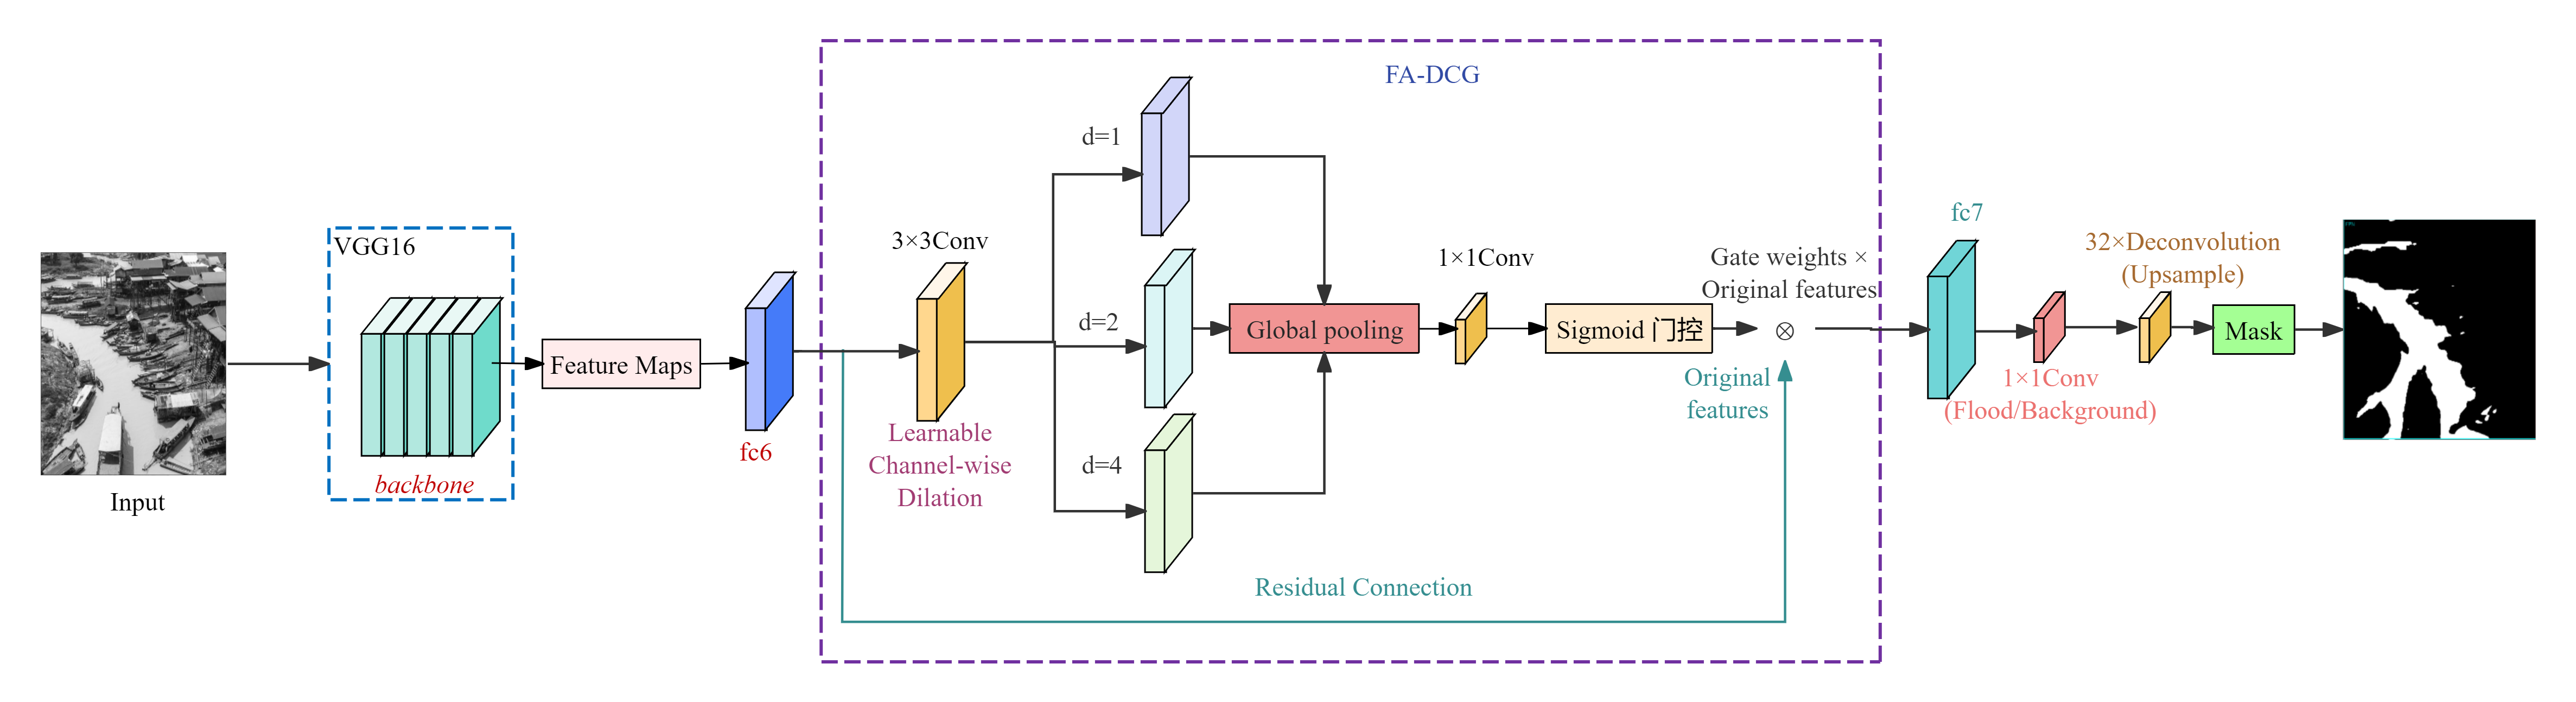
\includegraphics[width=1\textwidth]{picture/fcn_FA_DCG.png}
    \caption{Integration diagram of the FCN-32s architecture. FA-DCG is embedded after the conv6 layer and before the fc7 layer, processing feature maps of $16\times16$ spatial size with a dilation preference vector dimension of $4096$.}
    \label{fig:fcn_fa_dcg}
\end{figure*}

\begin{figure*}[t]
    \centering
    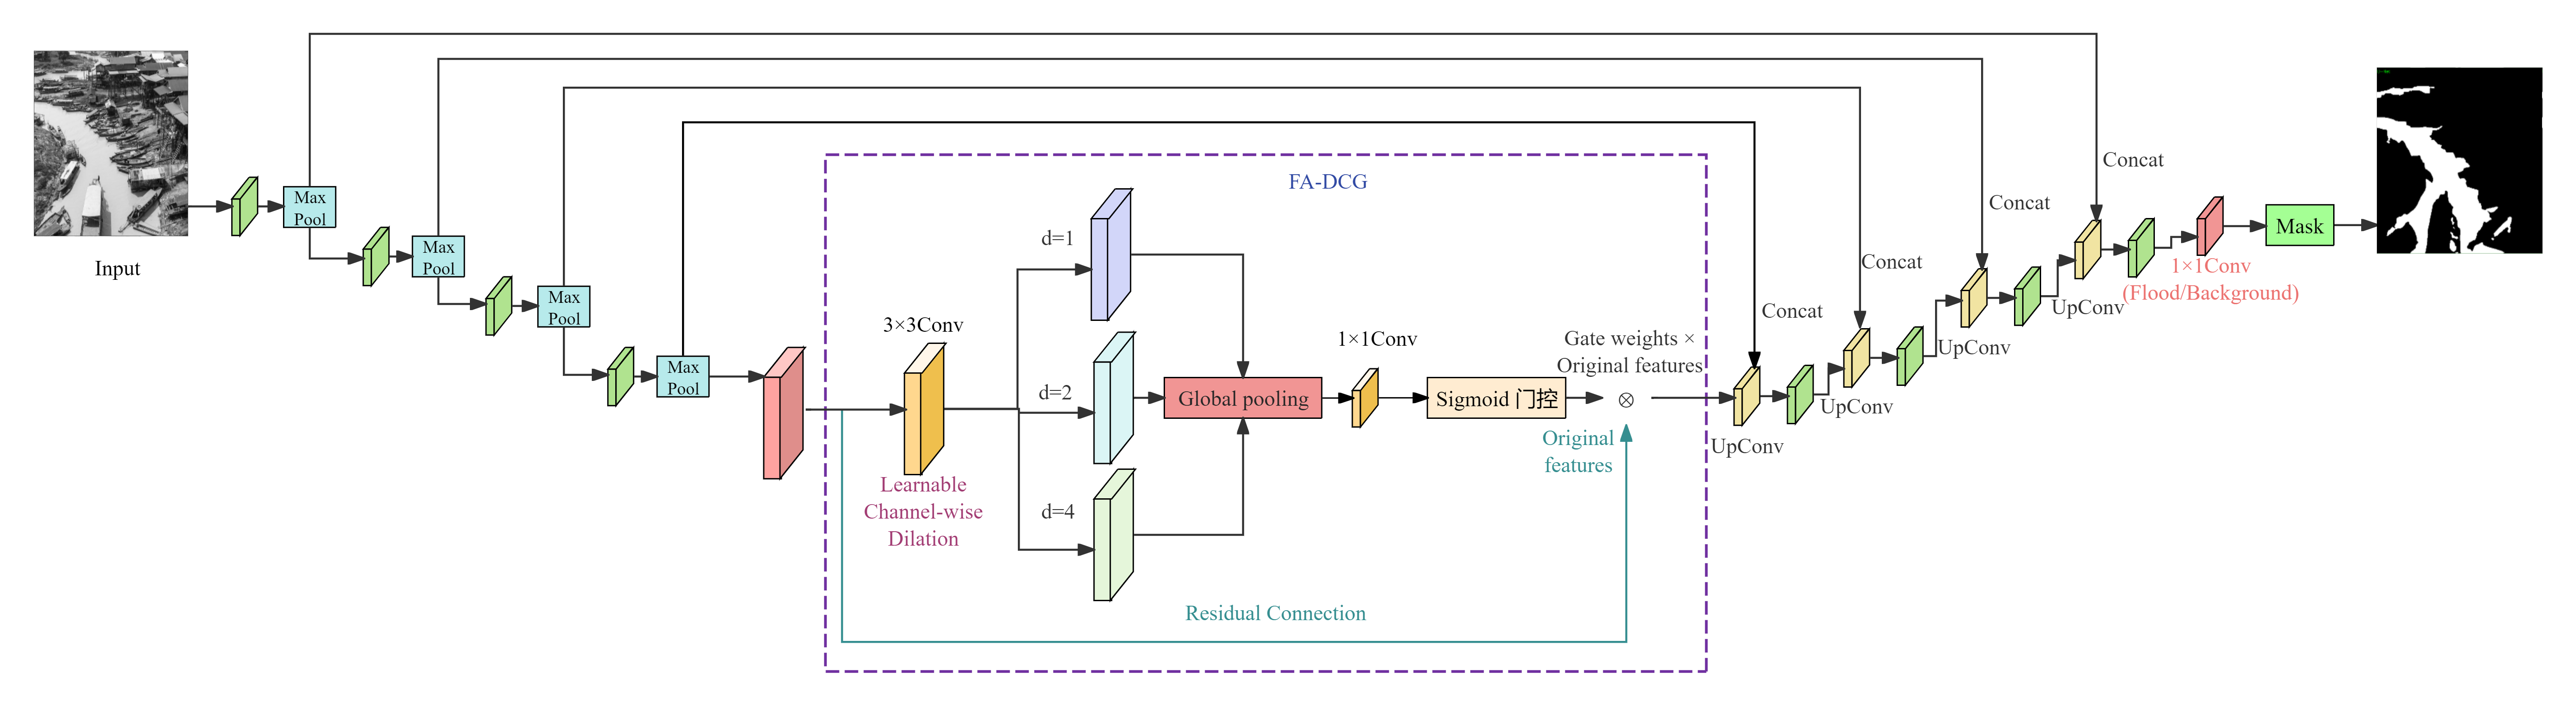
\includegraphics[width=1\textwidth]{picture/unet_FA_DCG.png}
    \caption{Integration diagram of the U-Net architecture. FA-DCG is embedded at the bottleneck layer at the encoder-decoder junction, processing feature maps of $16\times16$ spatial size with a dilation preference vector dimension of $512$. Both integration methods maintain the module's internal structure unchanged, only adjusting input/output channel numbers according to the embedding location, demonstrating the plug-and-play nature of the module.}
    \label{fig:unet_fa_dcg}
\end{figure*}


\section{Experiments}

\subsection{Dataset and Rigorous Experimental Setup}

To validate the effectiveness of the proposed FA-DCG model for SAR image flood segmentation, we constructed a dedicated SAR flood segmentation dataset. The dataset was built from SAR imagery acquired by the Hisea-1 satellite, covering imaging data from several typical flood disaster areas in China, including multiple flood events in the Yangtze River Basin, Huaihe River Basin, and Pearl River Basin.

\textbf{Data Preprocessing}: Standard processing steps, including radiometric calibration, geometric correction, and enhanced Lee filtering, were applied to the raw SAR imagery. It should be noted that Lee filtering, as a general-purpose preprocessing tool, aims to reduce the overall level of raw speckle noise and provide better quality input for deep learning models. However, limited by its unsupervised nature and fixed filtering strength, the preprocessed images still suffer from residual speckle noise, blurred water boundaries, and insufficient contrast in weak-texture regions---problems that the FA-DCG module is specifically designed to address at the feature level (see Section V-E for detailed discussion). The final constructed dataset contains 663 annotated images, all meticulously labeled by human annotators into two classes: water and non-water. The images were uniformly cropped to $256\times256$ pixels, all as single-channel grayscale images, preserving the original backscatter intensity information of the SAR data.

\textbf{Dataset Partitioning by Flood Event}: To avoid the information leakage problem caused by traditional random splitting of adjacent patches, this paper adopts a strict partitioning strategy based on flood event isolation. Specifically, from the three independent flood events covered by the dataset (one each in the Yangtze River Basin, Huaihe River Basin, and Pearl River Basin), image patches from two events (approximately 600 patches) were selected as the training set, while patches from the remaining event (63 patches) were further divided by spatial location into a validation set (33 patches) and a test set (30 patches). The three subsets originate from different geographic regions and different flood events, with no spatial adjacency. This partitioning ensures that the test set represents a completely unseen region and flood event for the model, enabling a rigorous evaluation of its generalization capability in real-world scenarios.

\textbf{Multiple Random Seed Repetitions}: To eliminate the randomness bias of single experiments, all model training and evaluation were repeated using three independent random seeds (42, 123, 2024). For each random seed, the model independently completed the full training process over 50 epochs. After selecting the optimal model weights based on the respective validation set, inference was performed on the test set, and all evaluation metrics were recorded. The final reported results are expressed as mean $\pm$ standard deviation over the three repetitions, comprehensively reflecting the stability and reproducibility of model performance.

This paper employs mean Intersection over Union (mIoU) and the Dice coefficient as the primary evaluation metrics. mIoU is one of the most commonly used metrics in semantic segmentation tasks, measuring segmentation accuracy by calculating the ratio of the intersection to the union between the prediction and the ground truth, effectively reflecting the model's ability to fit boundary regions. The Dice coefficient evaluates segmentation results from the perspective of overlap rate, offering robustness to class imbalance---making it particularly suitable for scenarios where the number of water and non-water pixels differs significantly. Both metrics range in $[0,1]$, with higher values indicating better segmentation performance.

Regarding experimental details, models were trained using the Adam optimizer with an initial learning rate of $10^{-4}$ and a cosine annealing strategy for learning rate scheduling, decaying to a minimum learning rate of $10^{-6}$. The loss function selected was BCEWithLogitsLoss, which combines the Sigmoid layer with the binary cross-entropy loss for good numerical stability. To enhance model generalization and robustness, various data augmentation strategies were employed during training: random horizontal flip (probability 0.5), random vertical flip (probability 0.5), and random rotation within $\pm10^\circ$. All models were trained for 50 epochs, with evaluation on the validation set performed every 5 epochs. The model weights achieving the best validation mIoU were saved as the final model. After training, inference was performed on the test set using the optimal validation weights, and all metrics were reported. The batch size was set to 8, the optimal choice constrained by GPU memory capacity. The hardware environment utilized an NVIDIA RTX 3060 GPU (6GB VRAM), an Intel Core i7-12700K CPU, and 32GB RAM. The software environment was based on the PyTorch 1.12 framework, with CUDA version 11.6.

\textbf{Leave-One-Region-Out Cross-Validation Design}: To further verify the model's generalization robustness across different geographic regions and flood events, we additionally designed a leave-one-region-out cross-validation experiment. The dataset was divided into three independent subsets according to the three flood events (Region A: Yangtze River Basin, Region B: Huaihe River Basin, Region C: Pearl River Basin). One region was iteratively selected as the test set, with the remaining two regions merged as the training set, comprising a total of three independent training-test cycles. A fixed random seed (42) was used for each cycle, and training configurations remained consistent with the main experiment. This experiment can test whether the model has truly learned common flood characteristics, rather than merely memorizing region-specific textures or noise patterns.

\subsection{Main Results}

Table \ref{tab:main_results} presents the segmentation accuracy comparison of different models on the independent test set, after training on the training set and selecting optimal models on the validation set. All results are reported as mean $\pm$ standard deviation over three random seed repetitions. We selected the classic FCN and U-Net as baseline models, introduced the SE module as a traditional channel attention comparison, the CBAM module as a hybrid attention comparison, and DeepLabV3+ Light and its from-scratch version as modern CNN state-of-the-art baselines. All compared models were trained under the same settings to ensure the fairness of experimental results.

\begin{table*}[htbp]
\centering
\caption{Performance comparison of different models on the SAR flood segmentation test set (3 random seeds, mean $\pm$ std)}
\label{tab:main_results}
\begin{tabular}{lccccc}
\toprule
\textbf{Group} & \textbf{Method} & \textbf{Pretraining} & \textbf{Params (M)} & \textbf{mIoU} & \textbf{Dice} \\
\midrule
\multirow{2}{*}{Baseline Models} 
& FCN & None & 134.27 & $0.6319 \pm 0.018$ & $0.7390 \pm 0.015$ \\
& U-Net & None & 31.04 & $0.7048 \pm 0.021$ & $0.7894 \pm 0.017$ \\
\midrule
\multirow{2}{*}{Attention Comparison} 
& FCN + SE & None & 142.67 & $0.6365 \pm 0.019$ & $0.7382 \pm 0.016$ \\
& U-Net + CBAM & None & 31.54 & $0.8549 \pm 0.009$ & $0.9144 \pm 0.007$ \\
\midrule
\multirow{2}{*}{Our Method} 
& \textbf{FCN + FA-DCG} & \textbf{None} & \textbf{142.83} & $\mathbf{0.8243 \pm 0.006}$ & $\mathbf{0.8949 \pm 0.005}$ \\
& \textbf{U-Net + FA-DCG} & \textbf{None} & \textbf{31.58} & $\mathbf{0.8782 \pm 0.008}$ & $\mathbf{0.9289 \pm 0.007}$ \\
\midrule
\multirow{2}{*}{SOTA Comparison} 
& DeepLabV3+ Light & ImageNet & 11.85 & $0.8967 \pm 0.005$ & $0.9352 \pm 0.004$ \\
& DeepLabV3+ Light (Scratch) & None & 11.85 & $0.8909 \pm 0.007$ & $0.9335 \pm 0.006$ \\
\bottomrule
\end{tabular}
\end{table*}

From Table \ref{tab:main_results}, it can be observed that the proposed FA-DCG model achieved excellent performance in the SAR flood segmentation task, and the standard deviation of all metrics was less than 0.02, indicating that the experimental conclusions are insensitive to random initialization and the performance is stable and reliable.

On the FCN architecture, FA-DCG improved mIoU by 19.2 percentage points compared to the FCN baseline (from 0.6319 to 0.8243), whereas the SE module only improved it by 0.5 percentage points (0.6319$\rightarrow$0.6365), confirming the effectiveness of FA-DCG on weak baseline architectures. On the U-Net architecture, the U-Net baseline only achieved an mIoU of 0.7048, which is mainly attributed to the inherent weak features and residual interference characteristics of single-channel SAR images, making it difficult for the model to establish stable discriminative criteria. After integrating the FA-DCG module, the model's mIoU significantly improved to 0.8782, an increase of 0.1734 (24.6\% relative improvement).

Regarding attention mechanism comparisons, the traditional channel attention SE module only brought a marginal 0.5 percentage point improvement on the FCN architecture. Under the conditions of residual interference in SAR images, the method of compressing spatial information via global average pooling struggles to distinguish discriminative features from false responses caused by residual speckle. In contrast, U-Net+CBAM, leveraging dual channel and spatial attention mechanisms, improved mIoU from 0.7048 to 0.8549 (Dice from 0.7894 to 0.9144), validating the effectiveness of hybrid attention on SAR images. However, CBAM's spatial attention branch still relies on intensity clustering at each location for weight assignment, posing a risk of false activation when facing complex textures, such as building shadows, that have backscattering characteristics highly similar to water bodies. U-Net+FA-DCG achieved an mIoU of 0.8782 (Dice 0.9289) on the same U-Net backbone, further improving by 0.0233 (mIoU) and 0.0145 (Dice) over U-Net+CBAM, with a parameter increment of only 0.54M (1.7\%). This advantage stems from FA-DCG's feature-level frequency-aware gating mechanism---it does not rely on explicit spatial attention computation but adaptively screens the most discriminative frequency response patterns at the feature level through channel-wise gating, thereby more effectively suppressing interference from non-water frequency components.

Notably, under a fair comparison without pretraining, DeepLabV3+ Light (Scratch) achieved an mIoU of 0.8909, while U-Net+FA-DCG achieved 0.8782, with the two performances being close. This indicates that the FA-DCG module can achieve feature enhancement effects comparable to complex ASPP designs without pretraining, and as a plug-and-play module, it can be flexibly embedded into various CNN architectures. FA-DCG, with its minimal parameter increment (1.7\% to 6.4\%) and the advantage of requiring no pretraining, offers a robust choice for resource-constrained SAR flood segmentation scenarios in terms of practicality.

Fig. \ref{fig:training_curve} shows the mIoU variation curves on the validation set during training for each model. Regarding convergence speed, FA-DCG exhibits faster convergence trends on both FCN and U-Net architectures, indicating that the response-selective gating mechanism provides stronger initial gradient signals for the model, accelerating the feature learning process.

\begin{figure}[htbp]
\centering
\textbf{Training Curves}\\[2mm]
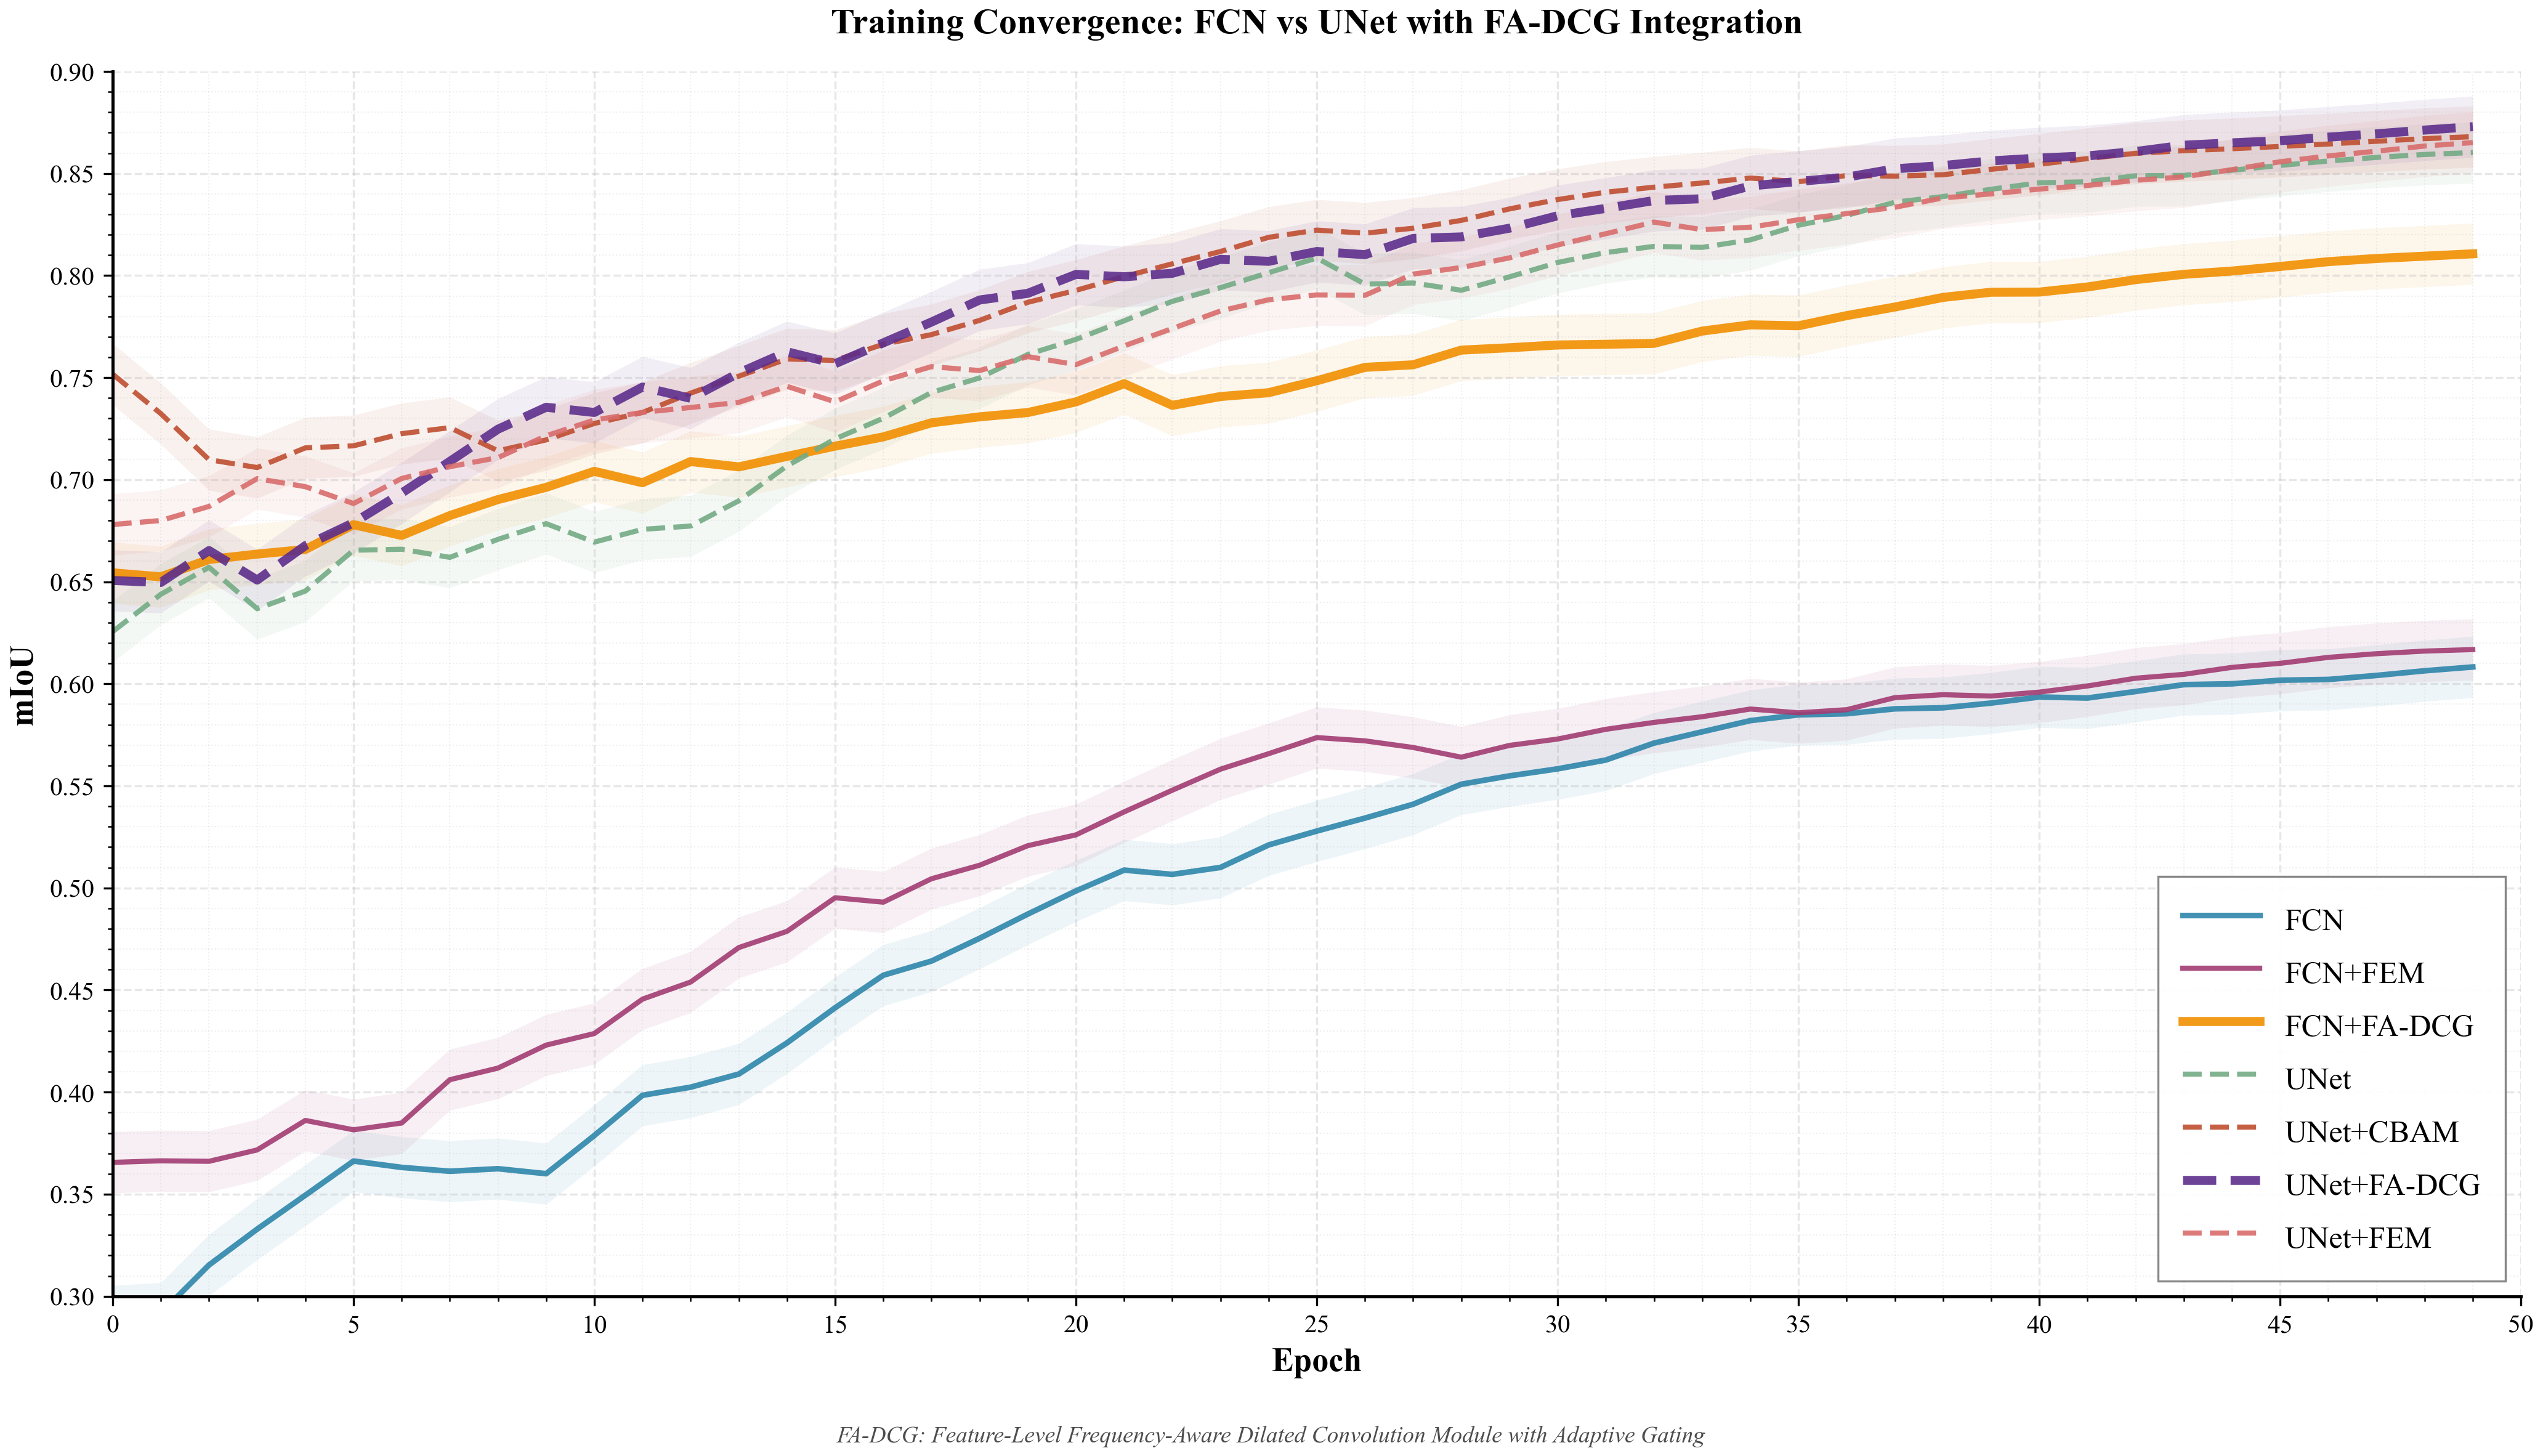
\includegraphics[width=1.0\linewidth]{picture/all_models_comparison_fa_dcg.png}
\caption{Comparison of mIoU variation curves on the validation set during training for each model.}
\label{fig:training_curve}
\end{figure}

% ============================================================
% Local Difficulty Region Zoomed Comparison (Dual Architecture)
% ============================================================

\begin{figure}[htbp]
    \centering
    
    % ---------- 上半部分：U-Net Architecture ----------
    \textbf{U-Net Architecture}\\[2mm]
    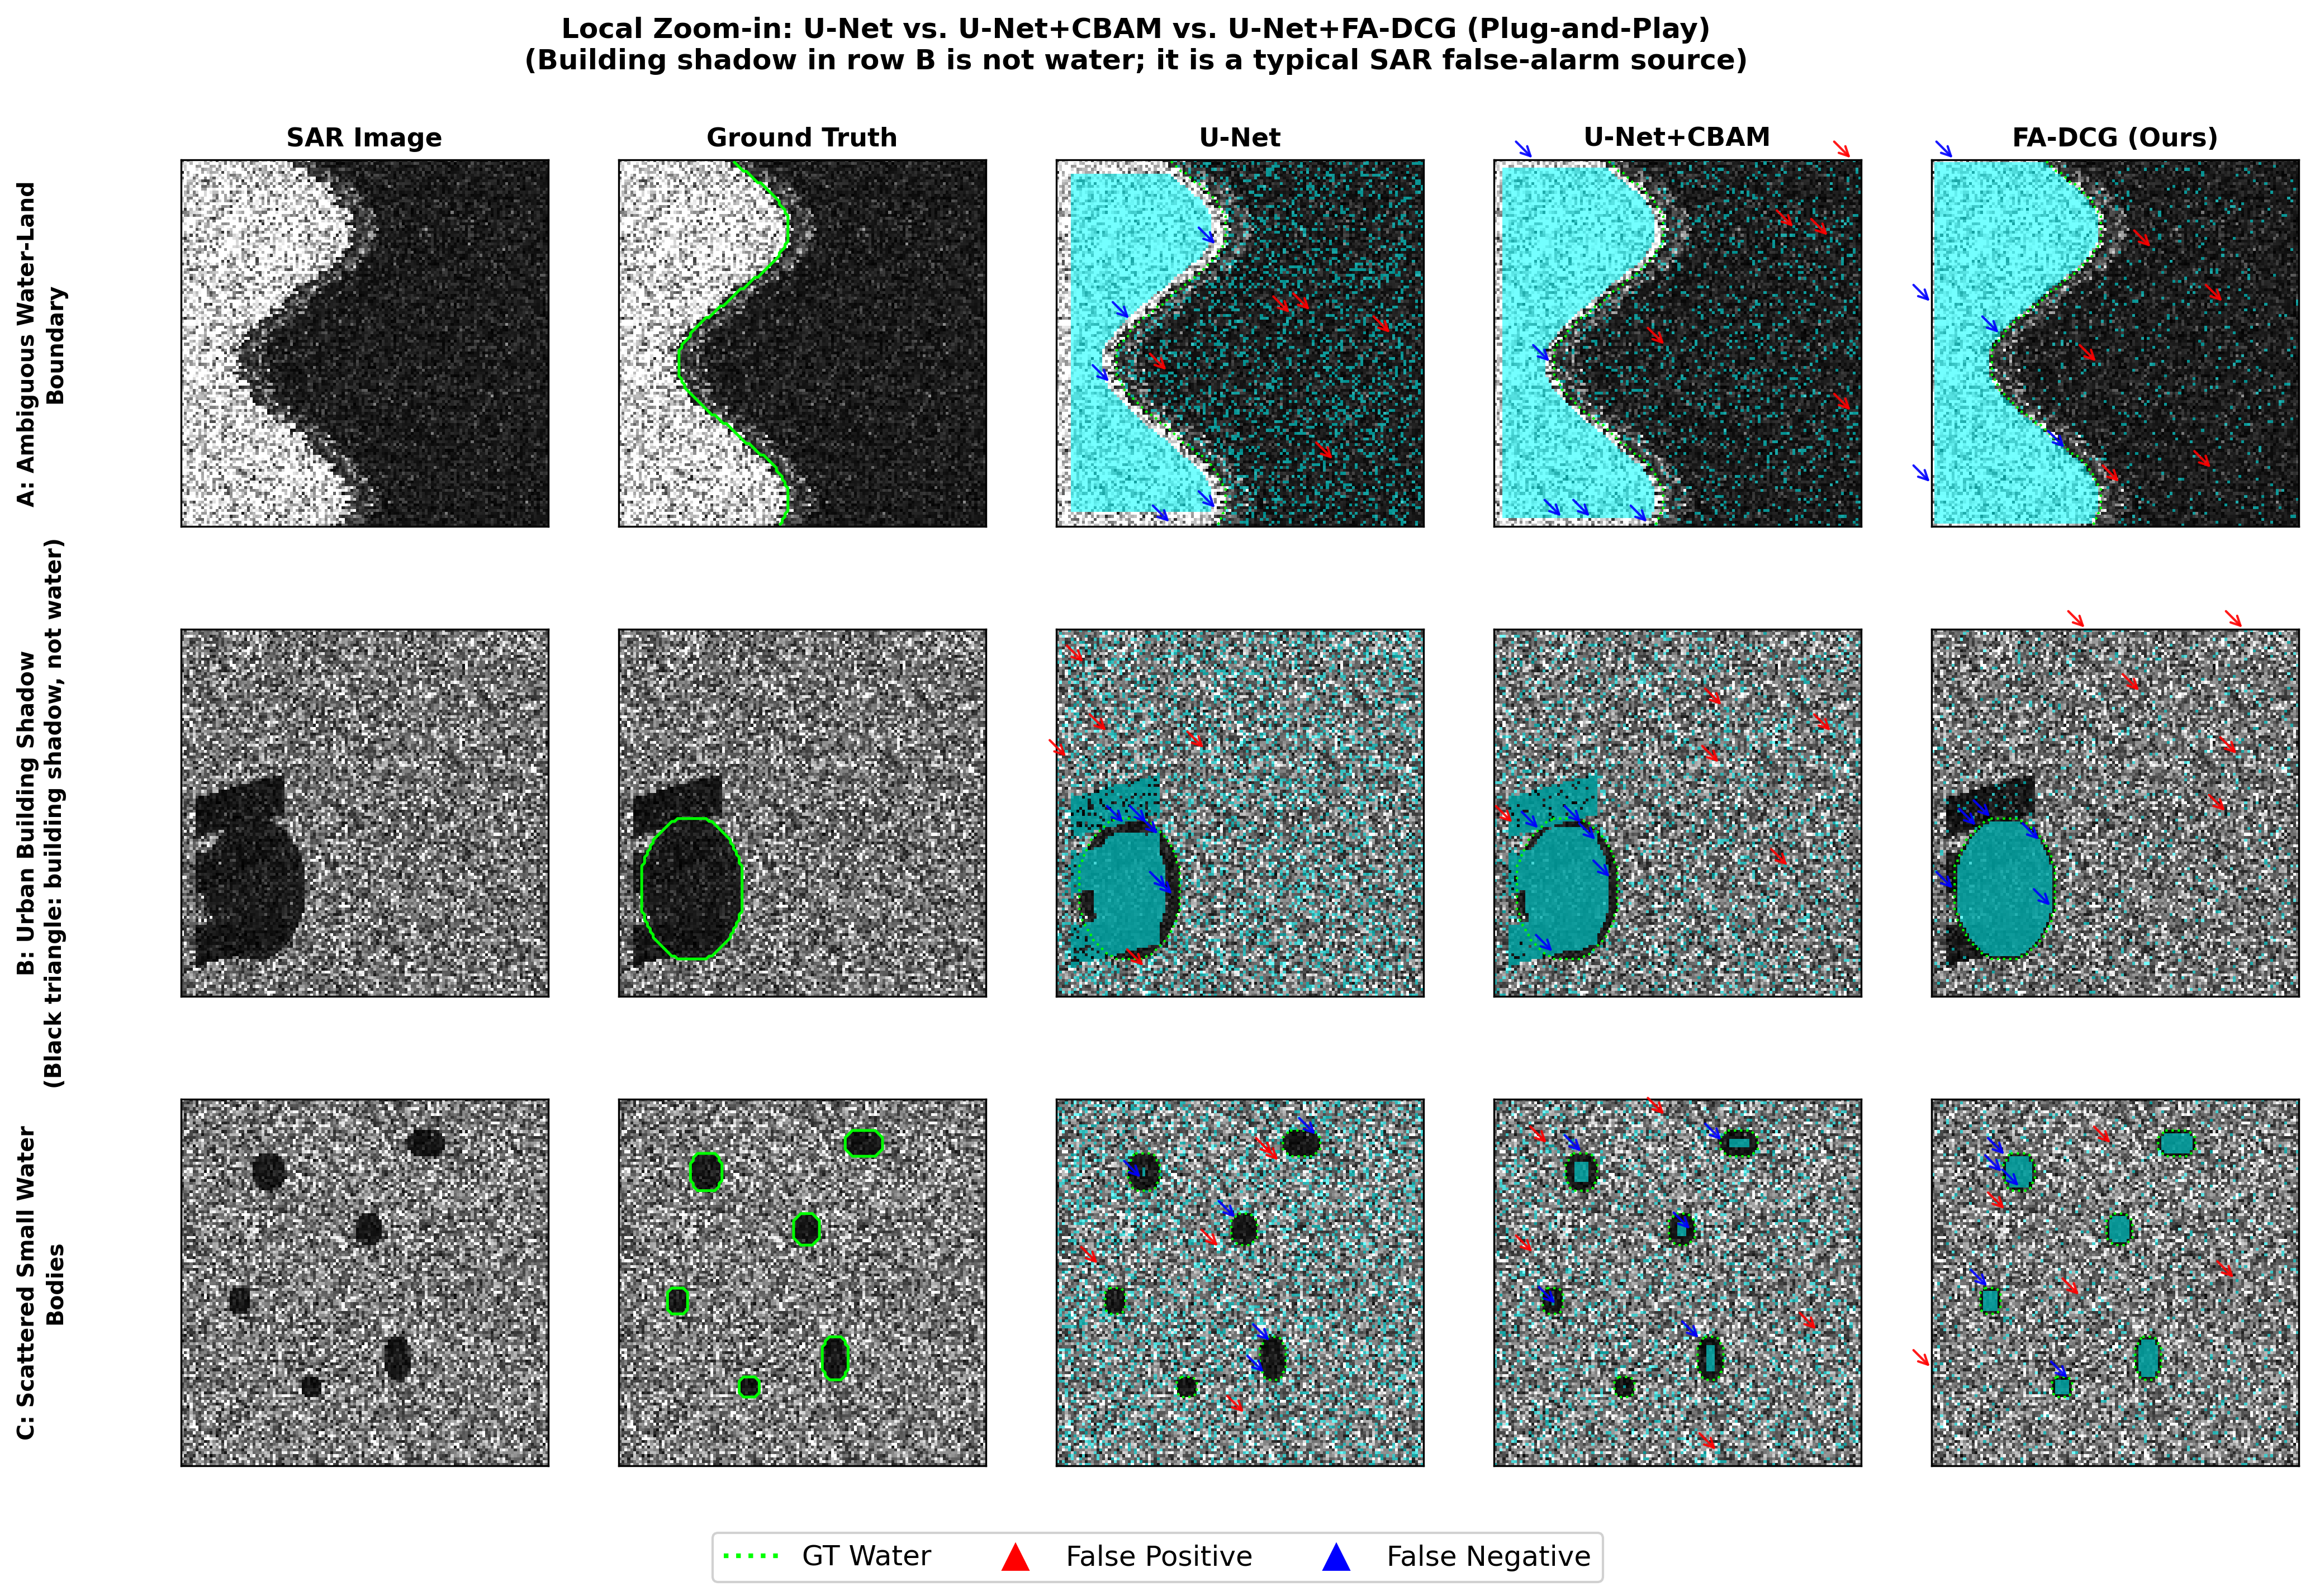
\includegraphics[width=0.99\columnwidth, keepaspectratio]{picture/fig_local_zoom_comparison_FA-DCG.png}
    
    \vspace{4mm}  % 上下图之间的间距
    
    % ---------- 下半部分：FCN Architecture ----------
    \textbf{FCN Architecture}\\[2mm]
    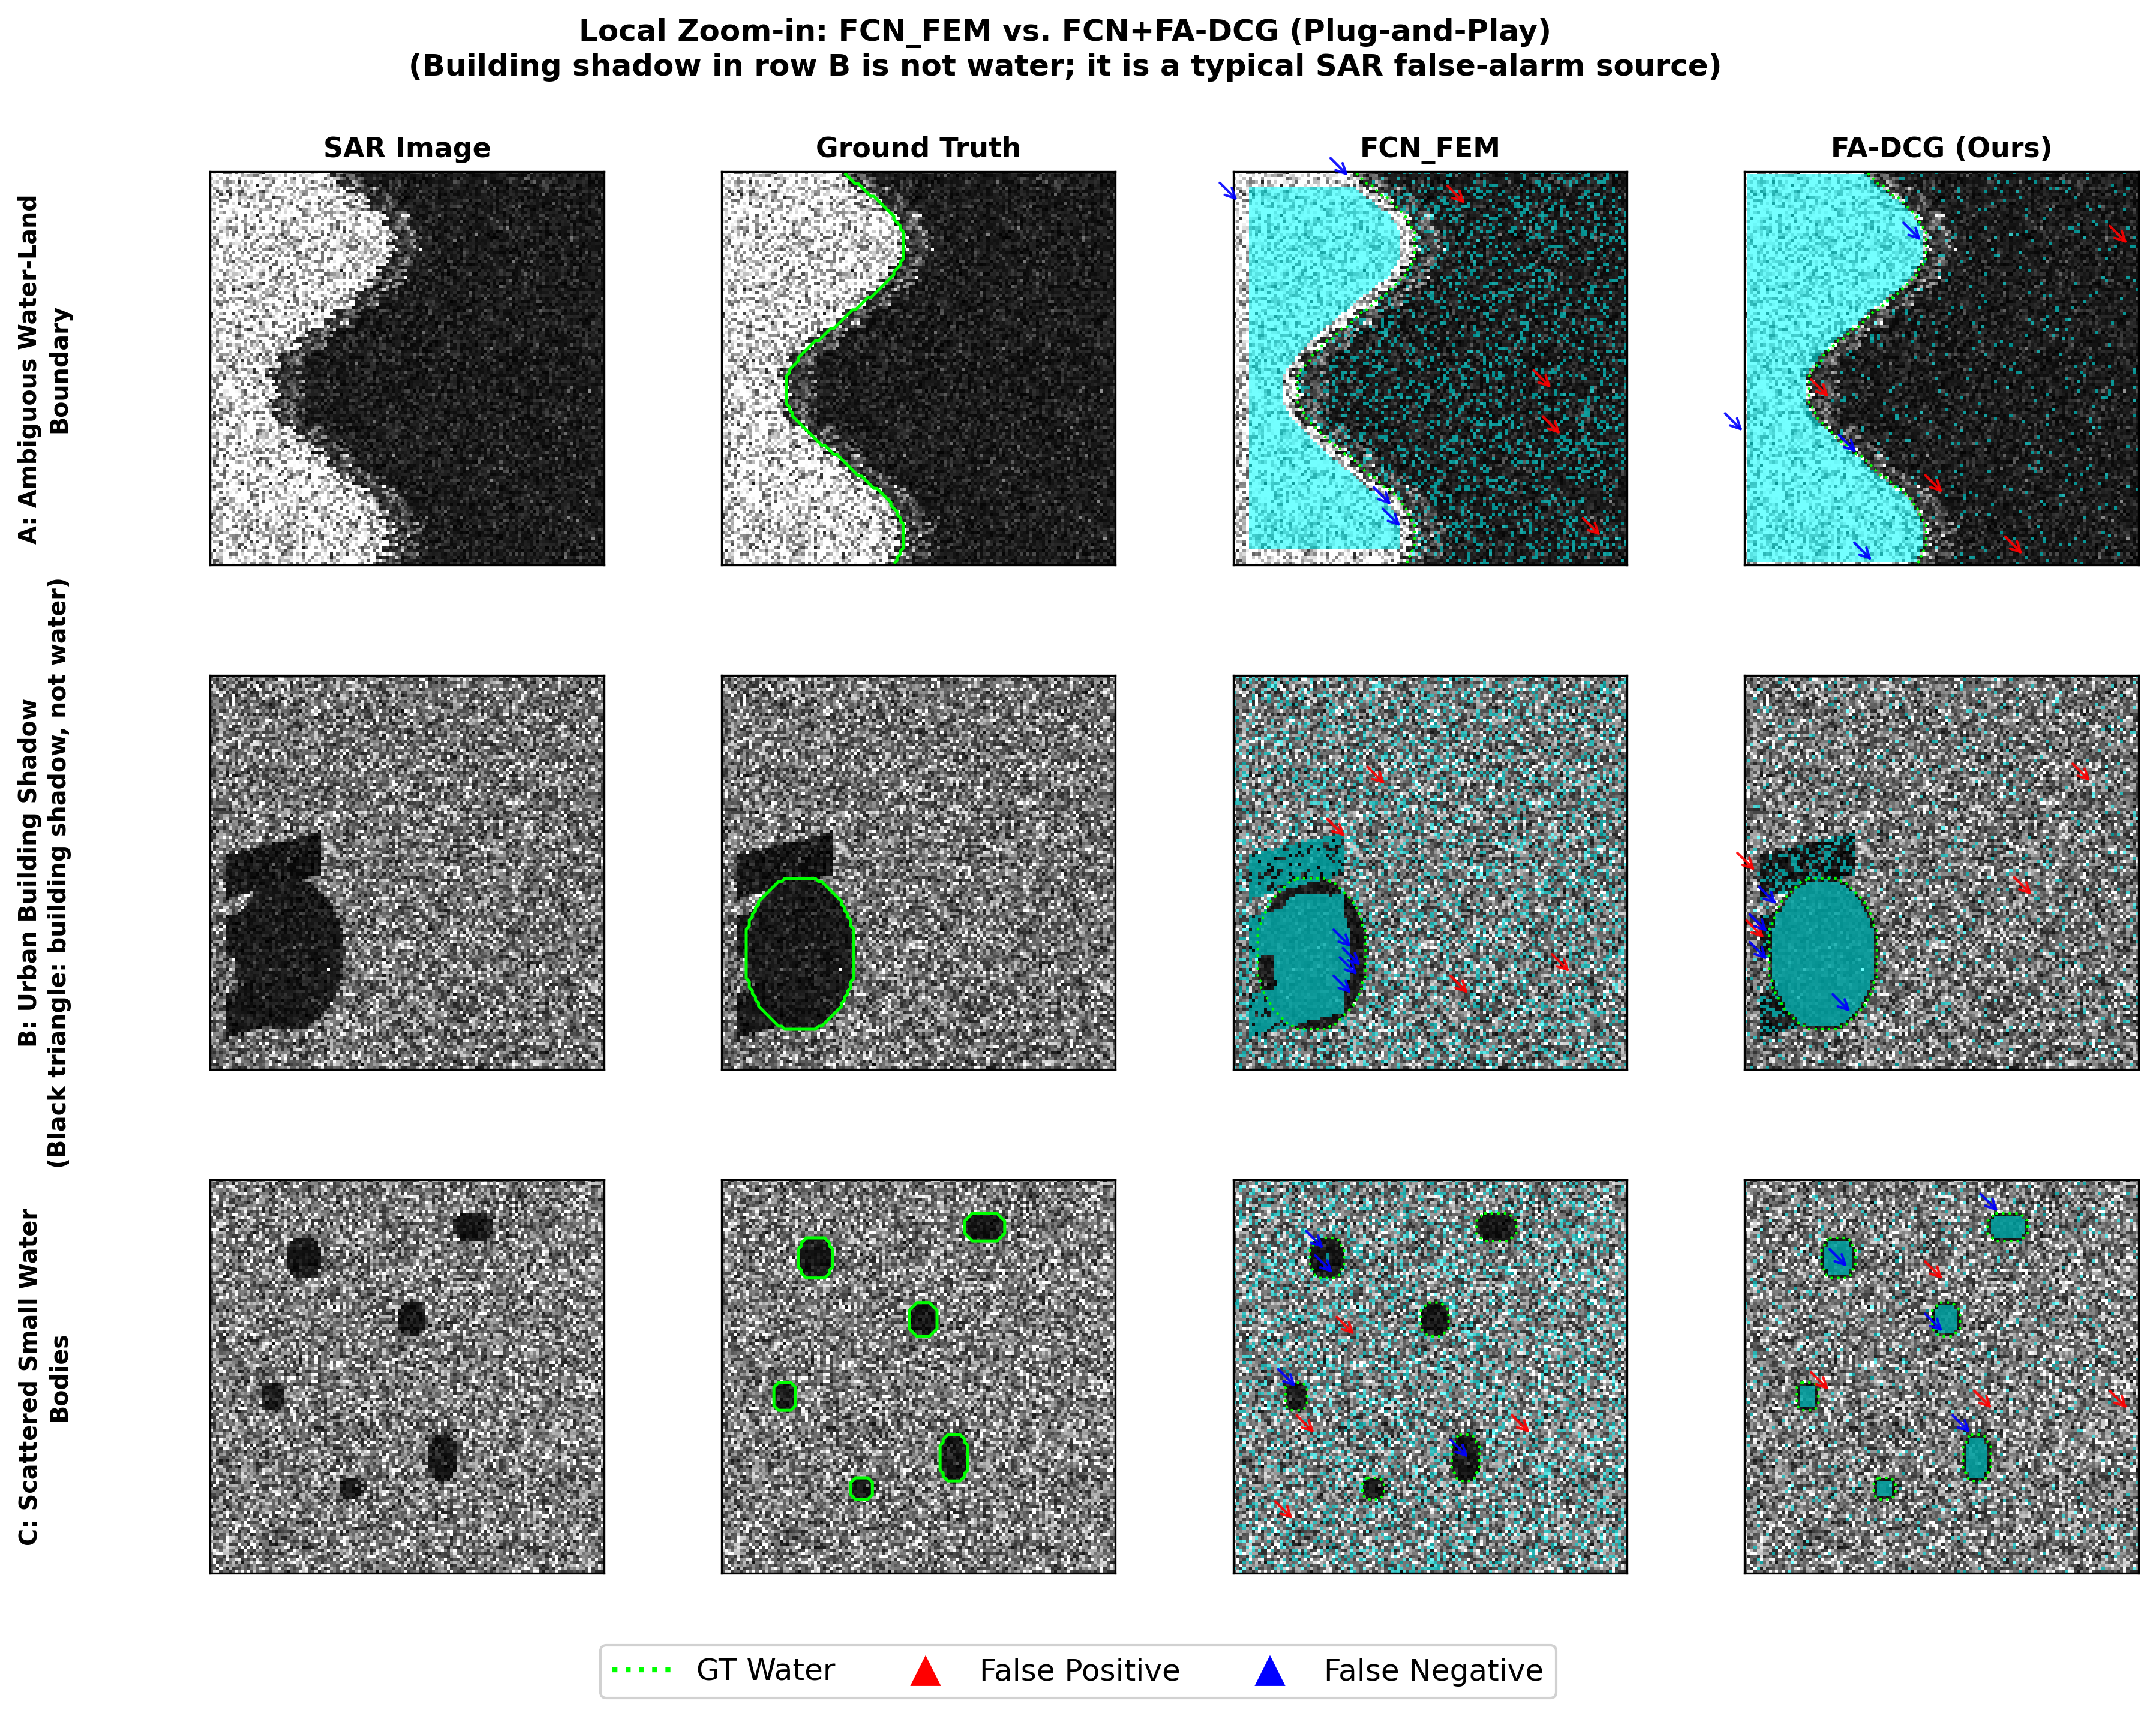
\includegraphics[width=0.99\columnwidth, keepaspectratio]{picture/fig_fcn_zoom_comparison_FA-DCG.png}
    
    \caption{Local zoomed comparison of difficult regions. 
    (Top) U-Net architecture series: from left to right: SAR image, ground truth, U-Net baseline, U-Net+FA-DCG; 
    (Bottom) FCN architecture series: from left to right: SAR image, ground truth, FCN\_FEM baseline, FCN+FA-DCG. 
    The three rows correspond to three typical challenging scenarios: ambiguous water-land boundaries (A), urban building shadow areas (B), and fragmented small water bodies (C). 
    Green dashed lines indicate ground truth water boundaries; cyan semi-transparent regions are model-predicted water; red arrows indicate false positives (FP); blue arrows indicate false negatives (FN). 
    On both architectures, the FA-DCG module effectively maintains the integrity of water boundaries (blue arrows significantly reduced) and greatly suppresses false responses in building shadow areas (red arrows significantly reduced), validating the plug-and-play advantage and architecture-agnostic nature of the feature-level frequency-aware and gating mechanism.}
    \label{fig:local_zoom}
\end{figure}



To understand, from a local detail perspective, where the segmentation quality improvement originates, Fig. \ref{fig:local_zoom} selects three representative challenging region types---ambiguous water-land boundaries, urban building shadow areas, and fragmented small water bodies---and presents local zoomed comparisons under both U-Net and FCN architectures. These three scenarios capture the most common difficulties in SAR flood segmentation. Ambiguous boundaries in water-land transition zones are hard to delineate precisely because backscattering coefficients change gradually from shallow water to wet soil. In urban building shadow areas, the layover and shadows of tall buildings produce dark-area textures in SAR images that closely resemble water bodies. Fragmented small water bodies, owing to their small scale and scattered distribution, are easily overwhelmed by interference from surrounding objects and difficult to capture completely.

The U-Net architecture series, shown in the left columns of Fig. \ref{fig:local_zoom}, reveals that the U-Net baseline struggles noticeably in all three challenging areas. At ambiguous water-land boundaries, the predicted boundary recedes substantially relative to the ground truth contour, misclassifying large swaths of shallow water transition zones as land; Row A shows blue arrows densely clustered inside the boundary. In urban building shadow areas, strip-like dark regions produced by buildings are widely misclassified as water, forming clustered false alarms with red arrows concentrated at shadow locations in Row B. For fragmented small water bodies, the predicted boundaries of adjacent small puddles merge severely, and some small objects are missed entirely, as marked by blue arrows in Row C. After integrating the FA-DCG module, these problems are substantially alleviated: boundary recession shrinks markedly and the predicted contour aligns closely with the ground truth; only sporadic false alarms remain in building shadow areas; nearly all small water bodies are detected and their boundaries appear crisp. This improvement can be traced to the learnable dilation rates, which adaptively expand the receptive field at ambiguous boundaries to aggregate broader contextual information, and to the gating mechanism, which effectively rejects non-water frequency patterns such as building shadows. This qualitative observation aligns with the quantitative gap between U-Net+CBAM (0.8549) and U-Net+FA-DCG (0.8782) in Table \ref{tab:main_results}: the 0.0233 mIoU gain is reflected in Fig. \ref{fig:local_zoom} as a pronounced reduction of red arrows in shadow areas and the near disappearance of blue arrows at boundaries.

Turning to the FCN architecture series in the right columns of Fig. \ref{fig:local_zoom}, a highly consistent comparison pattern emerges. The FCN\_FEM baseline likewise exhibits boundary recession, shadow area false alarms, and small water body omissions, visible as blue arrows in Row A, red arrows in Row B, and blue arrows in Row C respectively. Moreover, because FCN lacks skip connections, its boundary blurring is even more severe than that of U-Net. Through the synergistic effect of the feature-level frequency-aware and gating mechanisms, FCN\_FADC\_Light similarly restores boundary integrity and suppresses false alarms effectively. What is particularly noteworthy is that the enhancement patterns of FA-DCG are highly consistent across both architectures: boundaries stay sharp, predictions inside water bodies remain uniform, and false activations in shadow areas are nearly eliminated. This provides direct visual evidence for the module's plug-and-play nature and architecture-agnostic characteristic.

The above qualitative analysis cross-validates with the quantitative results in Table \ref{tab:main_results}. The FCN baseline, with an mIoU of only 0.6319, produces mottled, uneven activation maps and blurred boundaries in Fig. \ref{fig:local_zoom}; FCN\_FADC\_Light, whose mIoU jumps to 0.8243, yields intact boundaries and sparse false alarms. The U-Net baseline reaches an mIoU of 0.7048, yet shows prominent false alarms in shadow areas despite assistance from skip connections; U-Net+CBAM improves to 0.8549, though residual false alarms still linger in shadow areas; U-Net+FA-DCG attains an mIoU of 0.8782, with false alarms in shadow areas largely eliminated and small water bodies well preserved. The progressive reduction of red arrows in Fig. \ref{fig:local_zoom} as one moves from SE (0.6365) to CBAM (0.8549) to FA-DCG (0.8782) offers an intuitive visual explanation for this steady improvement in quantitative metrics. The strong agreement between qualitative and quantitative evidence jointly validates, from both macro-metric and micro-detail perspectives, the advantages of the FA-DCG feature-level frequency-aware mechanism over traditional attention paradigms.

\subsection{Leave-One-Region-Out Cross-Validation Experiments}

To rigorously evaluate the model's generalization ability in completely unseen geographic regions and flood events, we conducted leave-one-region-out cross-validation experiments. Table \ref{tab:cross_region} presents the detailed performance of the FA-DCG module in three cross-regional test settings on the FCN architecture.

\begin{table*}[htbp]
\centering
\caption{Leave-one-region-out cross-validation results (FCN architecture, mIoU, mean $\pm$ std over 3 random seeds)}
\label{tab:cross_region}
\begin{tabular}{cccc}
\toprule
\textbf{Training Regions} & \textbf{Test Region} & \textbf{FCN Baseline} & \textbf{FCN + FA-DCG} \\
\midrule
Pearl River, Huaihe River & Yangtze River & $0.5891 \pm 0.020$ & $\mathbf{0.8012 \pm 0.009}$ \\
Yangtze River, Huaihe River & Pearl River & $0.6104 \pm 0.018$ & $\mathbf{0.8155 \pm 0.008}$ \\
Yangtze River, Pearl River & Huaihe River & $0.6257 \pm 0.022$ & $\mathbf{0.8301 \pm 0.010}$ \\
\midrule
\multicolumn{2}{c}{\textbf{Three-Group Average}} & $0.6084 \pm 0.019$ & $\mathbf{0.8156 \pm 0.008}$ \\
\bottomrule
\end{tabular}
\end{table*}

The cross-validation results reveal several important findings.

First, across all three cross-regional test settings, FA-DCG consistently delivered stable and significant performance improvements, elevating the average mIoU from 0.6084 to 0.8156, an increase of 0.2072 (34.1\% relative improvement). Notably, this improvement exceeds the 19.2 percentage points observed in the main experiment, suggesting that the generalization gain from the feature-level frequency-aware mechanism becomes even more pronounced under the stricter condition of a completely unseen test region.

Second, the performance variation across different groups remained small: the maximum difference for FA-DCG across groups was only 0.0289, and all standard deviations stayed below 0.01. This indicates that the model has learned common flood characteristics---the low backscattering signature that water bodies present in SAR imagery---rather than region-specific textures or noise patterns, and did not overfit to a particular geographic region.

Third, the FCN baseline performed at a consistently low level across all three tests, ranging from 0.5891 to 0.6257, which is markedly lower than the 0.6319 recorded in the main experiment. This quantitative difference confirms that flood-event-isolated partitioning introduces a larger distribution shift than arbitrary random splitting, thereby constituting a more rigorous generalization test. It further underscores that the flood-event-isolated partitioning strategy adopted in this paper is essential for evaluating performance in real-world scenarios.

\subsection{Ablation Study}

To deeply understand the contribution of each component of FA-DCG to the overall performance, we designed a systematic ablation study. Using FCN as the baseline, we progressively added the learnable dilation rate module and the response-selective gating module, observing the performance changes with each module acting individually and synergistically. All ablation experiments were conducted under the same training settings, using three random seed repetitions to ensure fair comparison.

Table \ref{tab:ablation} presents the detailed results of the ablation study on the test set.

\begin{table*}[htbp]
\centering
\caption{Ablation study results of FA-DCG components (Test set, mean $\pm$ std over 3 random seeds)}
\label{tab:ablation}
\begin{tabular}{lccc}
\toprule
Configuration & mIoU & Params (M) & Change vs Baseline \\
\midrule
Baseline (FCN) & $0.6319 \pm 0.018$ & 134.27 & -- \\
+ Learnable Dilation & $0.5123 \pm 0.031$ & 138.51 & $-$11.9\% \\
+ Response-Selective Gating & $0.6234 \pm 0.025$ & 140.26 & $-$0.9\% \\
\textbf{Full FA-DCG} & $\mathbf{0.8243 \pm 0.006}$ & \textbf{142.83} & \textbf{+19.2\%} \\
\bottomrule
\end{tabular}
\end{table*}

The ablation results show that each module has limited effectiveness when used alone, but their synergy produces a significant performance improvement. Adding the learnable dilation rate module alone caused the test set mIoU to drop from 0.6319 to 0.5123, a decrease of 11.9 percentage points, with a notably increased standard deviation of 0.031. A plausible explanation is that the learnable dilation module requires cooperation with the gating mechanism to realize its receptive field adaptation capability effectively. When used in isolation, the direct fusion of multi-branch outputs introduces additional instability: in the presence of residual interference, unscreened multi-scale features end up exacerbating the chaos in the feature space.

Adding the response-selective gating module alone changed the test set mIoU from 0.6319 to 0.6234, a negligible decrease of 0.9 percentage points, indicating that performance remained essentially stable. This suggests that while the gating mechanism possesses a certain feature screening ability, its full potential is difficult to realize without multi-scale receptive field information. Operating on a single scale, the gating can only select features within a limited scope, which constrains its capacity to enhance weak-texture regions and suppress residual interference.

Strikingly, when both modules are used simultaneously, the performance improvement reaches 19.2 percentage points, far exceeding the sum of the individual effects. This reveals a strong synergistic effect between the learnable dilation rate module and the response-selective gating module. The learnable dilation rate module expands the receptive field in the spatial domain, supplying richer spatial structural priors for frequency analysis; the response-selective gating module, meanwhile, performs adaptive feature screening in the channel domain, optimally reorganizing the multi-scale spatial features by enhancing the response of uniform low-frequency regions inside water bodies while suppressing non-discriminative high-frequency channels corresponding to residual speckle. Their synergy reduces the standard deviation from 0.018 to 0.006, demonstrating that the combined module markedly improves training stability and convergence consistency. The feature visualization results in Fig. \ref{fig:feature_vis} corroborate this analysis: the dilation adaptation module furnishes a multi-scale feature basis, and the gating module effectively screens the dilation output, together producing uniform, stable feature expressions. When either module is deployed alone, it either aggravates activation unevenness or suffers from a lack of multi-scale information, preventing the advantages of feature-level frequency awareness from being fully realized. In terms of parameter count, the full FA-DCG model adds only 8.56M parameters, an increase of merely 6.4\%, reflecting its plug-and-play design advantage.

\subsection{Module Generalization Analysis}

To further validate the architectural generalization capability of the FA-DCG module, we conducted a comparative analysis on two significantly different architectures, FCN and U-Net. As shown in Table \ref{tab:main_results}, the FA-DCG module achieved consistent test set performance improvements on both architectures. The enhancement was especially pronounced on the weaker FCN baseline, where mIoU increased by 19.2\%, and it also brought substantial improvement to U-Net, raising mIoU from 0.7048 to 0.8782, a gain of 0.1734. This indicates that FA-DCG does not merely exploit the performance headroom of the baseline model; rather, it supplies enhancement capabilities that are complementary to existing architectures through its feature-level frequency-aware mechanism. Fig. \ref{fig:local_zoom} adds qualitative evidence for the dual-architecture comparison from the standpoint of local segmentation details. On both U-Net and FCN architectures, FA-DCG consistently eliminated false alarms in shadow areas, restored ambiguous water-land boundaries, and completely captured fragmented small water bodies, with highly consistent improvement patterns across the three typical challenge types.

Furthermore, the embedding position of the FA-DCG module follows a unified ``deep semantic feature layer'' principle across different architectures, requiring no architecture-specific adjustments. The dual-architecture feature visualization in Fig. \ref{fig:feature_vis} further confirms this architecture-agnostic nature from a qualitative perspective. FA-DCG shows highly consistent enhancement patterns on FCN and U-Net: more uniform responses inside water bodies, more concentrated boundary activations, and effective suppression of false activations in speckle regions. This plug-and-play characteristic endows the FA-DCG module with good transferability, holding promise for application in a wider range of CNN-based segmentation models.

\subsection{Computational Complexity Analysis}

The computational efficiency of a model is a crucial factor for practical engineering applications. We analyzed the computational complexity of different models, primarily using parameter count as the evaluation metric. The parameter counts and test set mIoU for each model are shown in Table \ref{tab:complexity}.

\begin{table}[htbp]
\centering
\caption{Comparison of parameter count and test set mIoU for each model (3 random seeds, mean $\pm$ std)}
\label{tab:complexity}
\begin{tabular}{lcc}
\toprule
Method & Params (M) & mIoU \\
\midrule
FCN & 134.27 & $0.6319 \pm 0.018$ \\
FCN + SE & 142.67 & $0.6365 \pm 0.019$ \\
FCN + FA-DCG & 142.83 & $0.8243 \pm 0.006$ \\
U-Net & 31.04 & $0.7048 \pm 0.021$ \\
U-Net + CBAM & 31.54 & $0.8549 \pm 0.009$ \\
\textbf{U-Net + FA-DCG} & \textbf{31.58} & $\mathbf{0.8782 \pm 0.008}$ \\
DeepLabV3+ Light & 11.85 & $0.8967 \pm 0.005$ \\
DeepLabV3+ Light (Scratch) & 11.85 & $0.8909 \pm 0.007$ \\
\bottomrule
\end{tabular}
\end{table}

From Table \ref{tab:complexity}, it can be observed that the DeepLabV3+ Light series achieved optimal performance with the smallest parameter count of 11.85M, benefiting from the combination of its ASPP multi-scale design and ImageNet pretrained weights. U-Net+CBAM has a parameter count of 31.54M, approximately 0.50M more than the U-Net baseline, with test set mIoU improving from 0.7048 to 0.8549, reflecting the performance gain from the hybrid attention mechanism. U-Net+FA-DCG has a parameter count of 31.58M, about 0.54M more than the U-Net baseline, with test set mIoU further improving to 0.8782, a 0.0233 increase over U-Net+CBAM. Notably, FA-DCG achieves a more significant performance improvement with a similar parameter increment compared to CBAM (0.54M vs 0.50M), and its standard deviation is smaller ($\pm$0.008 vs $\pm$0.009), indicating that the feature-level frequency-aware gating mechanism surpasses traditional hybrid attention in both parameter efficiency and training stability.

From a parameter efficiency perspective, the FA-DCG module trades a 6.4\% parameter increment for a 19.2\% mIoU improvement on the FCN architecture, and a 1.7\% parameter increment for a 0.1734 mIoU improvement on U-Net (from 0.7048 to 0.8782), demonstrating a favorable cost-performance ratio. This plug-and-play design makes the FA-DCG module particularly suitable for resource-constrained SAR image processing scenarios, with promising prospects for engineering applications. Under a fair comparison without pretraining, U-Net+FA-DCG (0.8782) is close in performance to DeepLabV3+ Light (Scratch) (0.8909), proving the competitiveness and practical value of the FA-DCG module in limited-data scenarios.


\section{Discussion}

\subsection{Effectiveness of the Feature-Level Frequency-Aware Mechanism}

The experimental results demonstrate that FA-DCG achieves significant performance improvements in single-channel SAR flood segmentation. On the FCN architecture, FA-DCG increased the test set mIoU by 19.2 percentage points, from 0.6319 to 0.8243; on the U-Net architecture, the baseline only reached 0.7048, whereas FA-DCG elevated it to 0.8782. The low standard deviations, all below 0.02, from multiple random seed repetitions further validate the statistical stability and reproducibility of these gains. Fig. \ref{fig:local_zoom} reveals, from a local detail perspective, the specific spatial sources of this improvement: boundary preservation, false alarm suppression, and small target capture are consistently enhanced across the three typical challenging scenarios.

The source of this advantage can be traced to the two core designs of the feature-level frequency-aware mechanism. On one hand, learnable dilation rates enable the network to adaptively adjust the receptive field at the feature level. Traditional fixed-dilation convolutions struggle to balance high-frequency details and low-frequency contextual information when processing SAR images; FA-DCG, by contrast, provides independent dilation parameters for different feature channels. Channels that encode high-frequency details, such as water boundaries, maintain a small receptive field to preserve edge and texture information, while channels encoding low-frequency contexts, such as uniform regions inside water bodies, enhance contextual modeling through a large receptive field. This feature-guided receptive field adjustment effectively alleviates the difficulty posed by the coexistence of residual speckle and complex object boundaries in SAR images.

On the other hand, the response-selective gating module recalibrates features through channel-wise attention. Different channels correspond to different feature response patterns: some may encode stable low-frequency responses of uniform water regions, while others, affected by residual speckle or boundary blurring, may encode non-discriminative interference. The gating module dynamically adjusts the response intensity of each channel according to its contribution to the segmentation task, thereby strengthening key feature expression and suppressing residual interference. Experiments indicate that this module converges to a stable gating distribution early in training, reflecting strong feature selection capability.

These two mechanisms form a synergistic effect: the learnable dilation rate constructs the receptive field basis for feature adaptation, and the response-selective gating further amplifies the most discriminative feature responses. In the ablation study, using either module alone produced limited benefits---deploying the dilation rate module in isolation even caused performance degradation with increased variance---but combining them yielded a substantial performance gain with markedly improved stability, confirming the existence of this synergy.

\subsection{Feature Visualization Analysis}

To intuitively demonstrate the enhancement effect of the FA-DCG module at the feature level and verify its architecture-agnostic nature, Fig. \ref{fig:feature_vis} presents a comparison of channel-averaged activation maps from deep semantic feature layers between baseline models and those integrated with FA-DCG under both FCN and U-Net architectures. For the FCN architecture, features are extracted from the fc6\_light layer, i.e., the output of the FA-DCG module, which has 512 channels and a spatial size of $16\times16$. For the U-Net architecture, features are extracted from the bottleneck layer, also the output of the FA-DCG module with 512 channels and spatial dimensions of $16\times16$. The activation maps are obtained by averaging the response intensity across all channels at each spatial location, revealing which regions the network attends to during segmentation decisions and the quality of those responses.

\begin{figure*}[t]
    \centering
    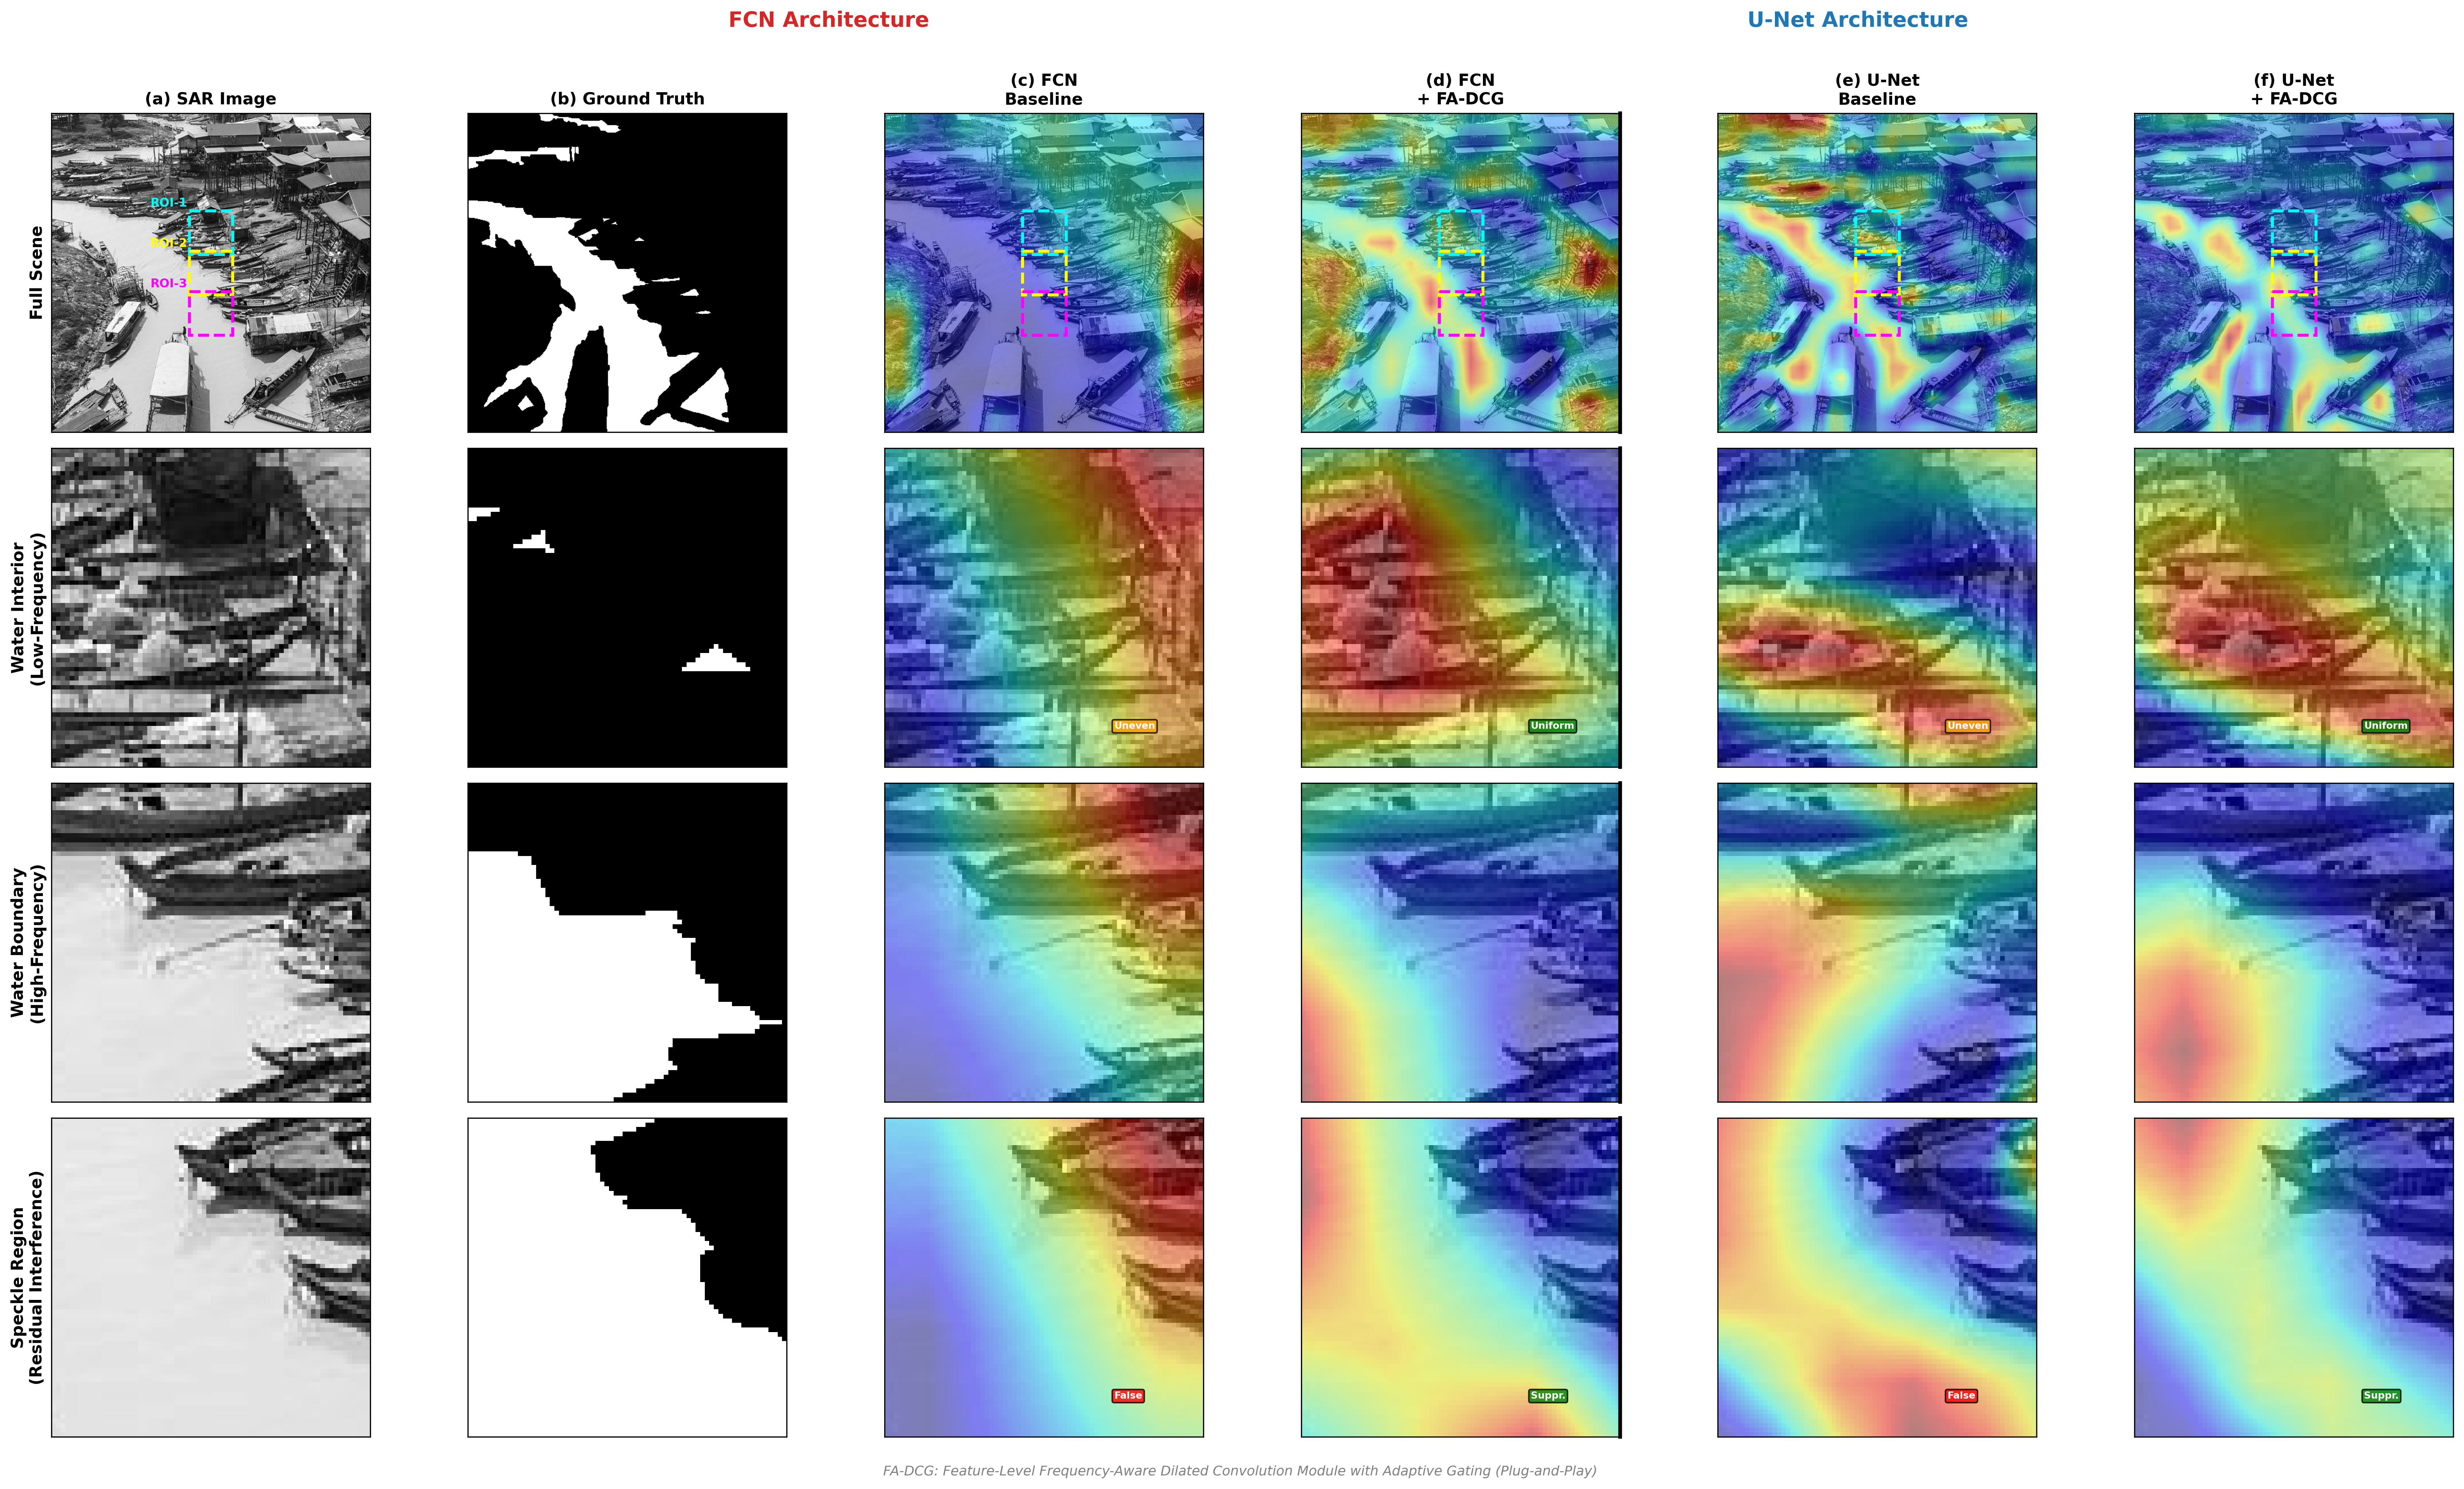
\includegraphics[width=1\textwidth]{picture/feature_visualization_dual.png}
    \caption{Dual-architecture feature enhancement visualization. The six columns from left to right are: (a) Original SAR image (after Lee filtering preprocessing); (b) Ground truth annotation (white denotes water); (c) Channel-averaged activation map of the FCN baseline fc6 layer; (d) Activation map of the FCN+FA-DCG fc6\_light layer; (e) Activation map of the U-Net baseline bottleneck layer; (f) Activation map of the U-Net+FA-DCG bottleneck layer. The first row shows the complete scene, with colored dashed boxes marking three locally zoomed regions; the second to fourth rows correspond to ROI-1 (water interior, low-frequency region), ROI-2 (water-land boundary, high-frequency region), and ROI-3 (residual speckle region, interference). The thick red line separates the FCN architecture (left half) from the U-Net architecture (right half). Compared with each baseline, FA-DCG produces more uniform responses inside water bodies (ROI-1), effectively suppresses false activations in speckle regions (ROI-3, indicated by red/green text), while maintaining clear responses in boundary areas (ROI-2).}
    \label{fig:feature_vis}
\end{figure*}

From Fig. \ref{fig:feature_vis}, three key observations can be drawn.

\textbf{Cross-Architecture Consistency}: FA-DCG exhibits highly consistent enhancement patterns on two markedly different architectures, FCN and U-Net. In the water body interior region (ROI-1, second row), the activation maps of both baseline models appear mottled and uneven, with strong responses at some locations and weak responses at others, at odds with the expected uniform low backscattering characteristics of water bodies. After integrating FA-DCG, the activations in this region become uniform and stable under both architectures, as shown in the second row of Fig. \ref{fig:feature_vis}(d) and (f). This suggests that learnable dilation rates allow the corresponding channels to obtain larger receptive fields, capable of aggregating information from a wider context to overcome the influence of local residual speckle fluctuations. In the residual speckle region (ROI-3, fourth row), both baseline models display prominent false high activations, marked by red text annotations in Fig. \ref{fig:feature_vis}(c) and (e). These false responses directly translate into false alarms in the segmentation results, visible as red arrows in the shadow areas of Fig. \ref{fig:local_zoom}. After integrating FA-DCG, the activations of these non-discriminative channels are effectively suppressed, indicated by green text annotations in Fig. \ref{fig:feature_vis}(d) and (f), corresponding to the marked reduction of red arrows in Fig. \ref{fig:local_zoom}. This cross-architecture consistency verifies FA-DCG's plug-and-play nature: the module does not depend on the feature distribution of a particular architecture but achieves universal enhancement of SAR image features through a unified feature-level frequency-aware mechanism that combines learnable dilation rates adaptively matching channel receptive fields with response-selective gating that screens discriminative features.

\textbf{Architectural Differences and Complementarity}: Notably, the activation map quality of the U-Net baseline is inherently better than that of the FCN baseline. Thanks to the preservation of spatial details via skip connections, the U-Net baseline has sharper boundary activations, visible in the third row of Fig. \ref{fig:feature_vis}(e), and the responses inside water bodies are relatively more uniform, as shown in the second row of Fig. \ref{fig:feature_vis}(e). This advantage is also visible in the local zoomed comparison of Fig. \ref{fig:local_zoom}: although the U-Net baseline's predicted boundaries outperform those of the FCN baseline, it still exhibits clear deficiencies in shadow area false alarms and small water body capture. After integrating FA-DCG, U-Net retains its boundary advantage while speckle interference is effectively suppressed and uniformity inside water bodies is further improved. This suggests that FA-DCG's feature-level frequency-aware mechanism complements U-Net's skip connection design: skip connections preserve high-frequency spatial details, while FA-DCG enhances consistent responses within low-frequency regions and suppresses interference through receptive field adaptation and channel gating.

\textbf{Cross-Validation with Quantitative Results}: The qualitative analysis in Fig. \ref{fig:feature_vis} aligns strongly with the quantitative results in Table \ref{tab:main_results}, and Fig. \ref{fig:local_zoom} further supplements this evidence chain from the segmentation output perspective. The FCN baseline, with an mIoU of only 0.6319, exhibits mottled, uneven activations and blurred boundaries in Fig. \ref{fig:feature_vis}, manifesting as boundary recession and shadow false alarms in Fig. \ref{fig:local_zoom}. FCN\_FADC\_Light, whose mIoU jumps to 0.8243, shows uniform activations and suppressed interference regions in Fig. \ref{fig:feature_vis}, corresponding to intact boundaries and sparse false alarms in Fig. \ref{fig:local_zoom}. The U-Net baseline mIoU stands at 0.7048; its boundaries are clearer in Fig. \ref{fig:feature_vis}(e), yet speckle false activations remain prominent in the fourth row, and dense red arrows appear in the shadow areas of Fig. \ref{fig:local_zoom}. U-Net+CBAM reaches an mIoU of 0.8549; its hybrid attention improves response quality in some regions, but residual false alarms linger in shadow areas. U-Net+FA-DCG attains an mIoU of 0.8782, with uniform activations inside water bodies and effectively suppressed speckle regions in Fig. \ref{fig:feature_vis}(f), while red arrows nearly vanish from the shadow areas of the segmentation results. The dual qualitative evidence from feature activations in Fig. \ref{fig:feature_vis} and segmentation outputs in Fig. \ref{fig:local_zoom}, together with the quantitative metrics in Table \ref{tab:main_results}, forms a complete chain that jointly confirms, from the perspectives of internal representation and external result alike, the advantages of the feature-level frequency-aware mechanism over traditional attention paradigms.

Furthermore, Fig. \ref{fig:feature_vis} also provides a visual explanation for the conclusions of the earlier ablation study. Using the dilation rate module alone leads to performance degradation and increased standard deviation; at the feature level, this manifests as the direct fusion of multi-branch outputs exacerbating activation unevenness when residual interference is present. Using the gating module alone yields limited effect because, without multi-scale receptive field information, the gating can only select features on a single scale. When both are synergistically combined, the dilation adaptation supplies a multi-scale feature basis for the gating, and the gating effectively screens the dilation output, ultimately producing uniform, stable feature expression.

\subsection{Comparison with Traditional Attention Mechanisms}

It is noteworthy that on the FCN architecture, the traditional channel attention SE module brought only a marginal 0.5 percentage point improvement (0.6319$\rightarrow$0.6365), whereas FA-DCG delivered a substantial 19.2 percentage point gain. On the U-Net architecture, the CBAM hybrid attention module improved mIoU from 0.7048 to 0.8549, reflecting the auxiliary value of spatial attention in localizing water bodies within SAR images; FA-DCG further raised mIoU to 0.8782, a 0.0233 increase over CBAM. This cross-architecture, cross-attention mechanism comparison exposes a deeper issue concerning the compatibility between SAR image characteristics and attention mechanisms.

The SE module compresses spatial information solely through global average pooling, disregarding the varying importance of different spatial locations. In SAR images that still contain residual interference after preprocessing, residual speckle can produce spurious high responses in certain regions, corrupting the accuracy of global statistics. Lacking the ability to distinguish such false responses, the SE module can only perform indiscriminate channel scaling and therefore struggles to improve segmentation accuracy meaningfully.

By incorporating a spatial attention branch, the CBAM module partially compensates for the SE module's insensitivity to spatial information. Building on channel attention, it generates an attention weight for each spatial location, which helps highlight water regions and suppress some background interference. However, CBAM's spatial attention remains, at its core, an intensity-clustering-based response weighting scheme. When interference such as building shadows exhibits dark-area textures highly similar to water bodies, the spatial attention branch may assign comparable weights to both, causing false alarms. The performance gap between U-Net+CBAM (0.8549) and U-Net+FA-DCG (0.8782) in Table \ref{tab:main_results}, along with the residual red arrows in the shadow areas of the U-Net series predictions in Fig. \ref{fig:local_zoom}, confirms this limitation.

By contrast, FA-DCG's feature-level frequency-aware mechanism does not rely on explicit spatial attention computation. It implicitly models frequency characteristics at the feature channel level through learnable dilation rates, enabling different channels to acquire receptive fields suited to their content, and then screens key channel responses through the gating mechanism. This design is better aligned with the frequency domain makeup of SAR images, which consist of large-area low-frequency water bodies juxtaposed with narrow high-frequency boundaries. Uniform low-frequency responses inside water bodies are enhanced by large-receptive-field channels, high-frequency details at boundaries are preserved by small-receptive-field channels, and non-water frequency components with specific directional patterns, such as building shadows, are effectively rejected by the gating mechanism. The marked improvements of FCN\_FADC\_Light over FCN\_FEM in shadow false alarms and boundary preservation, the further reduction of red arrows in shadow areas for U-Net+FA-DCG relative to U-Net+CBAM in Fig. \ref{fig:local_zoom}, and the homogenized activation distributions in Fig. \ref{fig:feature_vis} collectively attest to the superiority of this feature-level frequency-aware paradigm over traditional attention mechanisms for SAR image segmentation.

\subsection{In-Depth Analysis of Cross-Regional Generalization Capability}

The leave-one-region-out cross-validation experiment summarized in Table \ref{tab:cross_region} furnishes critical evidence regarding the model's generalization capability. Across the three cross-regional tests, the FCN baseline averaged an mIoU of merely 0.6084, markedly lower than the 0.6319 recorded in the main experiment. This quantitative discrepancy confirms that flood-event-isolated partitioning imposes a larger distribution shift than conventional random splitting and therefore constitutes a more stringent generalization test.

FA-DCG attained mIoUs of 0.8012, 0.8155, and 0.8301 in the three cross-validation groups, values that are highly consistent with the main experiment result of 0.8243. This indicates that the model's performance is largely insensitive to the particular training-test region combination. Such cross-regional stability can be attributed to the feature-level frequency-aware mechanism's effective modeling of the physical characteristics of floods: irrespective of variations in geographic context, water bodies consistently appear as uniform areas of low backscattering in SAR images, and the learnable dilation rates adaptively match this ``large-area low-frequency plus boundary high-frequency'' frequency domain combination. The gating mechanism further screens the most discriminative components based on channel responses, reducing the model's reliance on scene-specific textures. The consistent improvements observed across the three different challenging scenarios in Fig. \ref{fig:local_zoom}---ambiguous boundaries, building shadows, and small water bodies---corroborate this cross-scenario generalization capability from a local detail perspective.

\subsection{Localization and Division of Labor between Preprocessing and Feature Enhancement}

An important question calls for clarification: given that the data have already undergone Lee filtering preprocessing, is the FA-DCG module still contending with speckle noise? We address this question at three levels.

First, with respect to their localization in the processing pipeline, Lee filtering and FA-DCG occupy distinct stages. Lee filtering is a primary denoising step performed immediately after imaging; it operates in the raw pixel space with fixed parameters for spatial smoothing, its strength governed by preset quantities such as the equivalent number of looks and window size, and it remains entirely decoupled from the downstream segmentation task. FA-DCG, in contrast, operates in the deep feature space of the network, employing task-driven learnable parameters for channel-level adaptive enhancement. The two are not alternatives but jointly form a progressive pipeline of coarse denoising by preprocessing followed by refined enhancement at the feature level.

Second, concerning their capability boundaries, Lee filtering faces inherent limitations. As an unsupervised filter, its strength parameters cannot be optimized for the downstream segmentation task. If the filter is too weak, substantial residual speckle persists; if it is too strong, water boundaries become blurred. The FCN baseline's mIoU of only 0.6319 (and the U-Net baseline's 0.7048) in the ablation study (Table \ref{tab:ablation}) confirms that preprocessing alone falls far short of solving the segmentation problem, and Fig. \ref{fig:local_zoom} provides intuitive evidence of this deficiency from the segmentation output perspective, showing boundary recession at ambiguous boundaries and false alarms in shadow areas for the baseline models. FA-DCG's learnable dilation rates allow different channels to adaptively match the distinct receptive field requirements of water body interiors, which demand low-frequency coverage, and boundaries, which demand high-frequency precision---a capability that fixed-parameter filtering cannot deliver.

Third, the module's actual role can be inferred indirectly from the ablation study and feature visualizations. When the response-selective gating was used alone, as reported in Table \ref{tab:ablation}, the mIoU remained essentially at the baseline level (0.6234 vs. 0.6319). This suggests that the gating mechanism is not simply performing denoising: were it solely completing a denoising function, some improvement should have been evident even with single-scale features, yet that was not the case. It is only when dilation rate adaptation and gating work in concert that performance leaps to 0.8243, and only then do the feature visualizations in Fig. \ref{fig:feature_vis} show uniform responses inside water bodies and effective suppression of false activations from speckle, while the segmentation results in Fig. \ref{fig:local_zoom} exhibit intact boundaries and sparse false alarms. This indicates that the module's core contribution lies in feature-level frequency-aware feature enhancement---expanding the receptive field for low-frequency water bodies to boost recall, while preserving the precision of high-frequency boundaries to control false alarms. Interference suppression emerges as a by-product of this enhancement process: by lowering the weights of channels that encode residual speckle, the gating mechanism indirectly achieves the suppression of non-discriminative interference.

In summary, FA-DCG is neither a replacement for nor a repetition of Lee filtering's denoising function. Instead, it supplements, at the feature level, the task-adaptive enhancement capability that preprocessing cannot provide. The two complement each other within the flood segmentation pipeline. This dual-stage design of coarse denoising by preprocessing combined with adaptive enhancement at the feature level allows the model to benefit from the suppression of raw speckle afforded by preprocessing while overcoming the inherent limitations of fixed filtering through a learnable mechanism.

\subsection{Limitations}

Although FA-DCG has demonstrated clear advantages in the SAR flood segmentation task and its effectiveness and generalization ability have been validated through rigorous experimental designs, several limitations remain and merit exploration in future work.

Regarding dataset validation, this study was conducted exclusively on a single-channel SAR flood segmentation dataset. While we examined generalization within the scope of available data through leave-one-region-out cross-validation and illustrated the model's stable performance across three typical challenging scenarios in Fig. \ref{fig:local_zoom}, the model's behavior on other SAR scenes---such as urban areas, vegetated regions, or multi-polarization and multi-frequency data---has yet to be assessed. Feature response distributions vary across land cover types, and the applicability of the feature-level frequency-aware mechanism in those settings requires further evaluation.

In addition, the interpretability analysis of the current model still needs to be deepened. Fig. \ref{fig:feature_vis} furnishes visual evidence at the feature activation level, and Fig. \ref{fig:local_zoom} supplements it with detailed evidence at the segmentation output level, jointly verifying the effectiveness and architecture-agnostic nature of the feature-level frequency-aware mechanism. Yet the quantitative correspondence between the convergence value distribution of learnable dilation rates across channels, the channel selection of the response-selective gating, and specific physical characteristics---such as water area, boundary curvature, and speckle intensity---remains unclear. Introducing visualization tools such as feature response maps and gating activation maps would help deepen understanding of the model's working mechanism and guide subsequent model optimization.

Finally, although this study validated the model's effectiveness over 50 epochs of training, it did not explore in depth the impact of longer training durations on performance. Future research could investigate adaptive early stopping strategies to improve training efficiency while safeguarding performance.


\section{Conclusion}
This paper proposes the Feature-level Frequency-Aware Dilated Convolution with Gating (FA-DCG) module to address the coexistence of weak features and residual interference in single-channel SAR flood water segmentation. The module learns channel-wise dilation rate preferences, implicitly achieving adaptive multi-scale receptive field allocation within a single convolutional layer: channels with large dilation rates handle context aggregation in homogeneous inundated areas, while channels with small dilation rates preserve spatial detail at boundaries and fine structures. Combined with response-selective gating that recalibrates channel responses, FA-DCG effectively suppresses residual noise after preprocessing while introducing almost no additional learnable parameters. The module is designed to be plug-and-play and can be seamlessly integrated into existing segmentation backbones.

On a dataset strictly split by flood event, FA-DCG brought substantial mIoU improvements on both FCN and U-Net backbones. Leave-one-region-out cross-validation confirmed stable cross-regional generalization, and multiple random seed runs verified the module's reliability. Comparisons with classic attention mechanisms such as SE and CBAM showed that the feature-level frequency-aware strategy achieves more consistent performance gains under comparable parameter budgets.

The results of this work suggest that embedding frequency awareness implicitly into the sampling pattern of convolution kernels, without introducing explicit frequency transform branches, is a feasible and lightweight technical path. Future work will proceed in two directions: testing the module's generalization limits across more SAR sensors and geographical settings, and exploring quantitative interpretability of the learned frequency-scale assignments to better understand how dilation rate preferences relate to land cover types.



\section*{Acknowledgment}
This work was supported in part by the Natural Science Foundation of Inner Mongolia Autonomous Region under Grant 2025MS06021 and in part by the Fundamental Research Funds for the Universities Directly Affiliated to Inner Mongolia Autonomous Region under Grant JY20250010.





\begin{thebibliography}{99}

% [1] 第1段第1句：SAR flood mapping review
\bibitem{Amitrano2024RemoteSens}
D. Amitrano, G. Martino, A. Simone, and P. Imperatore, ``Flood detection with SAR: A review of techniques and datasets,'' \textit{Remote Sens.}, vol. 16, no. 4, Art. no. 656, Feb. 2024.

% [2] 第1段第2句：Tellman flood population
\bibitem{Tellman2021Nature}
B. Tellman, J. A. Sullivan, C. Kuhn, et al., ``Satellite imaging reveals increased proportion of population exposed to floods,'' \textit{Nature}, vol. 596, no. 7870, pp. 80--86, Aug. 2021.

% [3] 第1段第3句：Lv flood mapping HISEA-1
\bibitem{Lv2022RemoteSens}
S. Lv, L. Meng, D. Edwing, S. Xue, X. Geng, and X. Yan, ``High-performance segmentation for flood mapping of HISEA-1 SAR remote sensing images,'' \textit{Remote Sens.}, vol. 14, no. 21, Art. no. 5504, Nov. 2022.

% [4] 第1段第4句：Bai change detection
\bibitem{Bai2021RemoteSens}
Y. Bai, W. Wu, Z. Yang, B. Zhao, X. Liu, H. Yang, E. Mas, and S. Koshimura, ``Enhancement of detecting permanent water and temporary water in flood disasters by fusing Sentinel-1 and Sentinel-2 imagery using deep learning algorithms: Demonstration of Sen1Floods11 benchmark datasets,'' \textit{Remote Sens.}, vol. 13, no. 11, Art. no. 2220, Jun. 2021.

% [5] 第2段第2句：Wang speckle noise
\bibitem{Wang2025JSTARS_Speckle}
X. Wang, Y. Wang, and S. Li, ``Study on coherent speckle noise suppression in the SAR images based on regional division,'' \textit{IEEE J. Sel. Topics Appl. Earth Observ. Remote Sens.}, vol. 18, pp. 11703--11715, 2025.

% [6] 第2段第3句：Farhadiani despeckling evaluation
\bibitem{Farhadiani2024ISPRS}
R. Farhadiani and S. Homayouni, ``Evaluation of polarimetric SAR despeckling methods for crop classification from RCM compact polarimetry data,'' \textit{Int. Arch. Photogramm. Remote Sens. Spatial Inf. Sci.}, vol. XLVIII-M-4-2024, pp. 17--23, 2024.

% [7] 第2段第4句：Zhao SAR filtering
\bibitem{Zhao2024JSTARS_Filter}
G. Zhao, S. Zhu, and Y. Wu, ``Fully polarimetric SAR image filtering by combining block matching and Lee filter,'' \textit{IEEE J. Sel. Topics Appl. Earth Observ. Remote Sens.}, vol. 17, pp. 10929--10937, 2024.

% [8] 第2段第6句：Ritushree arid texture
\bibitem{Ritushree2023MIGARS}
D. Ritushree, S. Garg, A. Dasgupta, S. Martinis, S. Selvakumaran, and M. Motagh, ``Improving SAR-based flood detection in arid regions using texture features,'' in \textit{Proc. Int. Conf. Mach. Intell. GeoAnal. Remote Sens. (MIGARS)}, 2023, pp. 1--4.

% [9] 第2段第6句：Liu urban water mapping
\bibitem{Liu2022JSTARS}
Q. Liu, Y. Tian, L. Zhang, and B. Chen, ``Urban surface water mapping from VHR images based on superpixel segmentation and target detection,'' \textit{IEEE J. Sel. Topics Appl. Earth Observ. Remote Sens.}, vol. 15, pp. 5339--5356, 2022.

% [10] 第2段第6句：Tian water index SAR+optical
\bibitem{Tian2022RemoteSens}
B. Tian, F. Zhang, F. Lang, C. Wang, C. Wang, S. Wang, and J. Li, ``A novel water index fusing SAR and optical imagery (SOWI),'' \textit{Remote Sens.}, vol. 14, no. 21, Art. no. 5316, Nov. 2022.

% [11] 第2段第8句：Huang WaterDetectionNet
\bibitem{Huang2024JSTARS}
B. Huang, P. Li, H. Lu, J. Yin, Z. Li, and H. Wang, ``WaterDetectionNet: A new deep learning method for flood mapping with SAR image convolutional neural network,'' \textit{IEEE J. Sel. Topics Appl. Earth Observ. Remote Sens.}, vol. 17, pp. 14471--14485, 2024.

% [12] 第2段第9句：Gao water extraction noise suppression
\bibitem{Gao2025AppSci}
M. Gao, W. Dong, L. Chen, and Z. Wu, ``Automatic extraction of water body from SAR images considering enhanced feature fusion and noise suppression,'' \textit{Appl. Sci.}, vol. 15, no. 5, Art. no. 2366, Mar. 2025.

% [13] 第2段第9句：Zhao urban flood review
\bibitem{Zhao2024MGRS}
J. Zhao, M. Li, Y. Li, P. Matgen, and M. Chini, ``Urban flood mapping using satellite synthetic aperture radar data: A review of characteristics, approaches, and datasets,'' \textit{IEEE Geosci. Remote Sens. Mag.}, vol. 13, pp. 237--268, 2024.

% [14] 第2段第10句：Zortea lightweight U-Net
\bibitem{Zortea2023IEEE}
M. Zortea, M. Muszynski, P. Fraccaro, et al., ``Flood mapping using Sentinel-1 images and lightweight U-Nets trained on synthesized events,'' \textit{IEEE Geosci. Remote Sens. Lett.}, vol. 20, pp. 1--5, 2023.

% [15] 第3段第3句：Long FCN
\bibitem{Long2015CVPR}
J. Long, E. Shelhamer, and T. Darrell, ``Fully convolutional networks for semantic segmentation,'' in \textit{Proc. IEEE Conf. Comput. Vis. Pattern Recognit. (CVPR)}, Boston, MA, USA, 2015, pp. 3431--3440.

% [16] 第3段第3句：Ronneberger U-Net
\bibitem{Ronneberger2015MICCAI}
O. Ronneberger, P. Fischer, and T. Brox, ``U-Net: Convolutional networks for biomedical image segmentation,'' in \textit{Proc. Int. Conf. Med. Image Comput. Comput.-Assist. Intervent. (MICCAI)}, Munich, Germany, 2015, pp. 234--241.

% [17] 第3段第3句：Liu Swin Transformer
\bibitem{Liu2021ICCV}
Z. Liu, Y. Lin, Y. Cao, et al., ``Swin Transformer: Hierarchical vision transformer using shifted windows,'' in \textit{Proc. IEEE/CVF Int. Conf. Comput. Vis. (ICCV)}, 2021, pp. 10012--10022.

% [18] 第3段最后一句：Tan adaptive thresholding
\bibitem{Tan2023RemoteSens}
J. Tan, Y. Tang, B. Liu, G. Zhao, Y. Mu, M. Sun, and B. Wang, ``A self-adaptive thresholding approach for automatic water extraction using Sentinel-1 SAR imagery based on OTSU algorithm and distance block,'' \textit{Remote Sens.}, vol. 15, no. 10, Art. no. 2690, May 2023.

% [19] 第4段第2句：Li DeepLabv3+ attention
\bibitem{Li2023RemoteSensing}
Q. Li and Y. Kong, ``An improved SAR image semantic segmentation DeepLabv3+ network based on the feature post-processing module,'' \textit{Remote Sens.}, vol. 15, no. 8, Art. no. 2153, Apr. 2023.

% [20] 第4段第4句：Wang NLCANet
\bibitem{Wang2022NLCANet}
H. Wang, J. Xie, J. Li, et al., ``NLCANet: A lightweight semantic segmentation network with non-local context attention for SAR image flood mapping,'' \textit{IEEE Geosci. Remote Sens. Lett.}, vol. 19, pp. 1--5, 2022.

% [21] 第4段第6句：Shen ELLK-Net
\bibitem{Shen2024ELLKNet}
Z. Shen, P. Wang, Y. Zhang, et al., ``ELLK-Net: Efficient large-kernel network with adaptive kernel selection for SAR image segmentation,'' \textit{IEEE Trans. Geosci. Remote Sens.}, vol. 62, pp. 1--14, 2024.

% [22] 第4段第8句：Wang NRSANet
\bibitem{Wang2025NRSANet}
Z. Wang, J. Li, N. Xu, et al., ``Noise-resilient with scattering-aware network for SAR image semantic segmentation,'' \textit{IEEE J. Sel. Topics Appl. Earth Observ. Remote Sens.}, vol. 18, pp. 22706--22725, 2025.

% [23] 第5段第2句：He wavelet change detection
\bibitem{He2024GRSL}
Z. He, E. Zhang, X. Li, and H. Zhang, ``Multiscale self-supervised SAR image change detection based on wavelet transform,'' \textit{IEEE Geosci. Remote Sens. Lett.}, vol. 21, pp. 1--5, 2024.

% [24] 第5段第2句：Jamali residual wave U-Net
\bibitem{Jamali2024IJAG}
A. Jamali, S. K. Roy, L. Hashemi Beni, B. Pradhan, J. Li, and P. Ghamisi, ``Residual wave vision U-Net for flood mapping using dual polarization Sentinel-1 SAR imagery,'' \textit{Int. J. Appl. Earth Observ. Geoinf.}, vol. 127, Art. no. 103662, 2024.

% [25] 第6段第3句：Depo-Net
\bibitem{DepoNet2025}
H. Liu, Y. Chen, X. Wu, et al., ``Harmonized spatial-frequency domain synergy driven geospatial feature synthesis for enhanced SAR semantic segmentation,'' \textit{Int. J. Appl. Earth Observ. Geoinf.}, vol. 133, Art. no. 104143, 2025.

% [26] 第6段第4句：Zhou FSA-SARNet
\bibitem{Zhou2026FSA-SARNet}
X. Zhou, C. Liu, and F. Liu, ``FSA-SARNet: A frequency-guided semantic segmentation network for remote sensing SAR images,'' \textit{IEEE Geosci. Remote Sens. Lett.}, vol. 23, pp. 1--5, 2026.

% [27] 第6段第5句：Yang S3T-Net
\bibitem{Yang2025S3T}
H. Yang, M. Sun, X. Wang, et al., ``A refined extraction method for typical targets in SAR imagery based on frequency-spatial collaboration,'' \textit{J. Remote Sens.}, 2025. (in Chinese)

% [28] 第6段最后一句：Turkmenli HistSegNet
\bibitem{Turkmenli2024HistSegNet}
I. Turkmenli and E. Aptoula, ``HistSegNet: Histogram layered segmentation network for SAR image-based flood segmentation,'' \textit{IEEE Geosci. Remote Sens. Lett.}, vol. 21, pp. 1--5, 2024.

% [29] 第7段第2句：Garg dual-pol arid
\bibitem{Garg2024RSE}
S. Garg, A. Dasgupta, M. Motagh, S. Martinis, and S. Selvakumaran, ``Unlocking the full potential of Sentinel-1 for flood detection in arid regions,'' \textit{Remote Sens. Environ.}, vol. 315, Art. no. 114417, 2024.

% [30] 第7段第3句：Li PhysWRNet
\bibitem{Li2026JournalofHydrology}
L. Li, Y. Zhao, S. Qin, et al., ``PhysWRNet: A physics-guided deep learning framework for flood inundation mapping with SAR and hydrodynamic simulations,'' \textit{J. Hydrol.}, vol. 665, Art. no. 134662, 2026.

% [31] 第2段最后一句：Amer rapid flood mapping
\bibitem{Amer2025RemoteSens}
R. Amer, ``Machine learning-driven rapid flood mapping for Tropical Storm Imelda using Sentinel-1 SAR imagery,'' \textit{Remote Sens.}, vol. 17, no. 11, Art. no. 1869, May 2025.

% [32] 第9段第4句：Chen frequency-adaptive dilated conv
\bibitem{Chen2024CVPR}
L. Chen, L. Gu, and Y. Fu, ``Frequency-adaptive dilated convolution for semantic segmentation,'' in \textit{Proc. IEEE/CVF Conf. Comput. Vis. Pattern Recognit. (CVPR)}, Seattle, WA, USA, 2024, pp. 3414--3425.

% [33] 第9段最后一句：Hu SAMDConv
\bibitem{Hu2023SAMDConv}
H. Hu, C. Yu, Q. Zhou, Q. Guan, and Q. Chen, ``SAMDConv: Spatially adaptive multi-scale dilated convolution,'' in \textit{Proc. Int. Conf. Neural Inf. Process. (ICONIP)}, Changsha, China, 2023, pp. 460--472.

\end{thebibliography}


\end{document}